\documentclass[11pt,a4paper]{report}

\usepackage[utf8x]{inputenc}

\usepackage{mathpazo}
\usepackage{microtype}
\usepackage{graphicx}
\usepackage{verbatim}
\usepackage{url}
\usepackage{bm}
\usepackage{wrapfig}
\usepackage{float}
\usepackage{tocloft}
\usepackage{hyperref}

\usepackage{tikz}
\usetikzlibrary{intersections,through,calc}
\tikzset {>=stealth}


\textwidth=155mm
\textheight=230mm
\topmargin=0pt
\headheight=0pt
\oddsidemargin=0mm
\evensidemargin=0mm
\headsep=0pt
\parindent=0pt
\renewcommand{\baselinestretch}{1.15}
\setlength{\parskip}{0.3\baselineskip plus 1pt minus 1pt}
\addtolength{\jot}{3pt}

\graphicspath{{images/}}

\newcommand*{\disfrac}[2]{\displaystyle\frac{#1}{#2}}

\newcounter{project}

\newcommand*{\geoproject}[1]{%
  \refstepcounter{project}%
  \label{#1}%
  \hyperref[a.geogebra]{Geogebra Project~\theproject}%
}

%  Less space above chapter title
\makeatletter
\def\@makechapterhead#1{%
  {\parindent \z@ \raggedright \normalfont
    \ifnum \c@secnumdepth >\m@ne
        \centering\Large\bfseries \@chapapp\space \thechapter\par
        \hspace{.3em}
    \fi
    \Large \bfseries #1\par\nobreak
    \vskip 25\p@
  }}
\makeatother

%\includeonly{}

\begin{document}

% !TeX root = trigonometric-functions.tex

\hypersetup{pageanchor=false}
\thispagestyle{empty}

\vspace*{2ex}

\begin{center}


\textbf{\LARGE A Functional Approach to Teaching Trigonometry}

\bigskip
\bigskip
\bigskip
\bigskip

\textbf{\Large Avital Elbaum-Cohen and Moti Ben-Ari}

\bigskip
\bigskip

\url{http://www.weizmann.ac.il/sci-tea/benari/}

\bigskip

Version 0.2

\end{center}


\vfill

\begin{footnotesize}
\begin{center}
\copyright{}\ 2019 by Avital Elbaum-Cohen, Moti Ben-Ari, Department of Science Teaching, Weizmann Institute of Science.
\end{center}

This work is licensed under the Creative Commons Attribution-NonCommercial-ShareAlike 3.0 Unported License. To view a copy of this license, visit http://creativecommons.org/licenses/by-nc-sa/3.0/ or send a letter to Creative Commons, PO Box 1866, Mountain View, CA 94042, USA.
\end{footnotesize}

\bigskip

\begin{center}

\includegraphics[width=.15\textwidth]{../../by-sa.png}
\end{center}


\newpage
\setlength\cftbeforetoctitleskip{4ex}
\setlength\cftaftertoctitleskip{2ex}
\setlength\cftparskip{.3\baselineskip}

\tableofcontents
\thispagestyle{empty}


\newpage
\hypersetup{pageanchor=true}

\setcounter{page}{1}

\chapter{The Triangular and the Functional Approaches}

\section{Introduction}

We present an approach to teaching secondary-school trigonometry based upon functions instead of right triangles.
We offer pedagogical guidance including Geogebra projects.
The document is intended for teachers and those engaged in mathematical education who wish to become familiar with this approach and to use the learning materials that were developed.

Secondary-school mathematics textbooks typically present trigonometry in two contexts: (1) functions defined as ratios of the length of the sides of right triangles, and (2) functions of a real variable defined as the coordinates of points obtained by rotating a radius vector from the origin around the circumference of the unit circle.
The first context is closely connected with Euclidean geometry and, while the second context is closely connected with functions of a real variable, in particular, as they are studied in calculus.
The study of trigonometry provides a rare opportunity to use functions to solve problems having an applied aspect.
It is important to note that trigonometry can be studied independently in both contexts, so there seems to be no impediment to teaching and studying these chapters in either order.

Secondary-school students study of trigonometry only after studying the following topics:
\begin{itemize}
\item Euclidean geometry including circles and similar triangles.
\item Polynomial functions including tangents and derivatives.
\item Analytical geometry including the unit circle.
\end{itemize}

When using dynamic graphical software such as Geogebra in teaching, we must consider the best representation of the main feature we seek to demonstrate.
Technology allows us to create continuous and rapid change, which can leave a strong impression on the viewer, but the teacher must consider if the dynamic display enables the students to participate in a coherent mathematical discussion.

Chapter~\ref{ch.overview} introduces the triangular and functional approaches. Chapter~\ref{ch.pedagogy} presents a detailed plan for teaching the functional approach. Chapter~\ref{ch.translated} briefly discusses the functional approach for circles other than the unit circle at the origin. Chapter~\ref{ch.analysis} gives two proofs that $\sin' x=\cos x$, a geometric proof and an algebraic proof. Chapter~\ref{ch.additional} shows geometric definitions of the secant and cosecant functions, and the transitional from the functions to triangles. Appendix~\ref{a.geogebra} contains a table of links to the Geogebra projects (within the text, the projects are numbered). Appendix~\ref{a.simple} explains how the ``simple'' algebraic proof $\sin' x=\cos x$ is using the formula for $\sin (x+h)$ that itself has a ``complicated'' geometric proof.

% !TeX root = trigonometric-functions.tex

\chapter{Overview}\label{ch.overview}

\section{The triangular approach}

The \textit{triangular approach} (\cite{thompson}) defines the trigonometric functions as ratios between the lengths of the sides in a right triangle.
When you calculate the sine of an \emph{angle} as the ratio of the \emph{lengths} of the opposite side and the hypotenuse, there is a conceptual gap between the domain of the functions: angles measured in units such as radians, and the range of the functions which are are dimensionless real numbers obtained as ratios of lengths measured in units such as centimeters. This is usually not the case for functions studied in the calculus where the domain, the range and the calcutions are (dimensionless) real numbers.
Learning materials may not clarify the three different characteristics of the trigonometric functions.

Furthermore, students must learn the fundamental property of trigonometric functions that in every right triangle with the same acute angles, the  relations between sides remain constant. This is not easy but it is essential if the students are to be able to tell a coherent story about the meaning of the trigonometric functions defined on the domain of angles.

\begin{wrapfigure}[17]{r}{.45\textwidth}
\begin{center}
\vspace{-4ex}
%\includegraphics[width=.45\textwidth,keepaspectratio]{figure1}
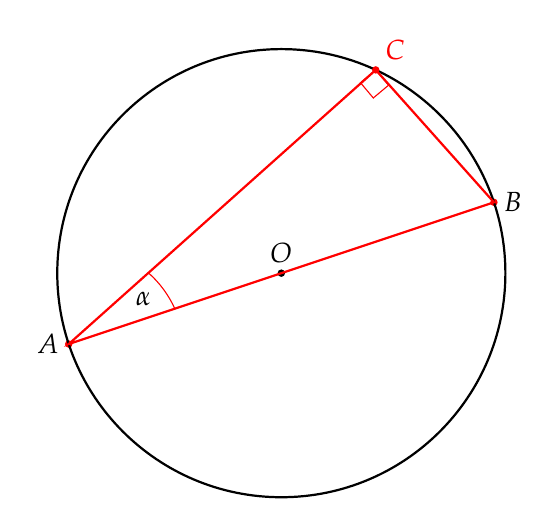
\begin{tikzpicture}[scale=.9]
  \coordinate[label = left:$A$]  (A) at (-3,-1);
  \coordinate[label = right:$B$] (B) at (3,1);
  \coordinate[label = above:$O$] (O) at (0,0);
  \fill[red] (A) circle (1.5pt);
  \fill[red] (B) circle (1.5pt);
  \fill (O) circle (1.5pt);
  \node[draw, thick, name path = circle] at (O)
    [circle through = (A)] {};
  \path[name path=side] (A) -- (60:4);
    \path [name intersections = {of = circle and side, by = {C}}];
  \fill[red] (C) circle (1.5pt) node[above right] {$C$};
  \draw[red,thick] (A) -- (B) -- (C) -- cycle;
  \draw[red,rotate=-140] (C) rectangle +(8pt,8pt);
  \draw[red] ($(A)+(15mm,14pt)$) arc[start angle=24,end angle=48,radius=15mm];
  \node at ($(A)+(30pt,18pt)$) {$\alpha$};
\end{tikzpicture}
\caption{Covariance of the angles and the sides in a right triangle. As you move point $C$, the acute angles and the lengths of the sides change.}\label{fig.covariance}
\end{center}
\end{wrapfigure}

Another difficulty with the triangular approach is that the functions are defined on an open domain $0^\circ<\alpha<90^\circ$.
It can difficult to understand the behavior of the sine and cosine functions in this context, for example: When are they ascending and when are they descending? Dynamic geometric constructions are required.

Consider a circle: all triangles with one vertex on the circumference whose angle subtends the diameter are right triangles (Figure~\ref{fig.covariance}, \geoproject{g.covariance}). As the point $C$ is moved along the circumference, the hypotenuse (the diameter of the circle) is unchanged, while the lengths of the sides vary so that trigonometric functions of the two acute angles remain correct.

Another potential difficulty with the triangular approach results from the default measurement of angles in units of degrees. We will expand on this  difficulty below.

Despite these potential difficulties we do not rule out beginning with the triangular approach.
To the contrary, this approach should be part of every teacher's repertoire, but these difficulties should be kept mind, so that students are presented with a coherent story.

\section{The functional approach}

In the \emph{functional approach}, trigonometric functions are defined on the unit circle where the independent variable is the amount of rotation around the circumference.
A rotation can be measured in degrees or radians (positive if the rotation is counterclockwise, negative if the rotation is clockwise).
The value of a rotation which is the number of degrees (or radians) between a ray from the origin and the ray that defines the positive $x$-axis.
The values of the functions cosine and sine are the projections of the intersection point of the ray and the unit circle on the $x$- and $y$-axes. The functions tangent and cotangent are determined by the intersections of the ray with tangents to the circle (Figure~\ref{fig.trig-functions}, \geoproject{g.definition-of-trig-functions}). 

\begin{wrapfigure}[20]{i}{.55\textwidth}
%\begin{figure}[htbp]
\begin{center}
\vspace{-2ex}
%\includegraphics[width=.45\textwidth,keepaspectratio]{figure2}
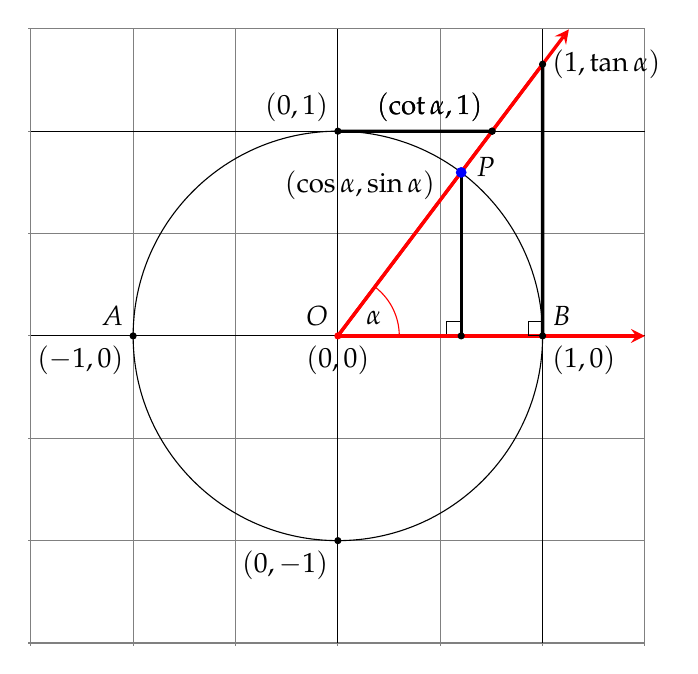
\begin{tikzpicture}[scale=.65]
\draw[step=2cm,white!50!black,thin] (-6.05,-6.05) grid (6,6);
\draw[thin] (-6,0) -- (6,0);
\draw[thin] (0,-6) -- (0,6);
  \coordinate[label = above left:$A$]  (A) at (-4,0);
  \coordinate[label = above right:$B$] (B) at (4,0);
  \coordinate[label = above left:$O$] (O) at (0,0);
  \node[below] at (O) {$(0,0)$};
  \node[draw, name path = circle] at (O)
    [circle through = (A)] {};
  \draw[red,very thick,name path=side,->] (O) -- (53:7.5);
  \draw[name path=tangent] (4,-6) -- (4,6);
  \path [name intersections = {of = circle and side, by = {C}}];
  \draw[very thick] (C) -- (C |- O) coordinate (CS);
  \draw[rotate=90] (CS) rectangle +(8pt,8pt);
  \path [name intersections = {of = side and tangent, by = {T}}];
  \draw[red,very thick] (O) -- (T);
  \draw[very thick,->,red] (O) -- (6,0);
  \draw[rotate=90] (B) rectangle +(8pt,8pt);
  \draw[name path=cotangent] (-6,4) -- (6,4);
  \draw[red] ($(O)+(12mm,0pt)$) arc[start angle=0,end angle=53,radius=12mm];
  \node at ($(O)+(20pt,10pt)$) {$\alpha$};
  \path [name intersections = {of = side and cotangent, by = {CT}}];
  \draw[very thick] (B) -- (T);
  \draw[very thick] (CT) -- (0,4);
  \fill (A) circle (2pt) node[below left] {$(-1,0)$};
  \fill (B) circle (2pt) node[below right] {$(1,0)$};
  \fill[red] (O) circle (2pt);
  \fill (CT) circle (2pt) node[above left] {$(\cot \alpha,1)$};
  \fill (CS) circle (2pt);
  \fill (CT) circle (2pt) node[above left] {$(\cot \alpha,1)$};
  \fill[blue] (C) circle (3pt) node[black,right,xshift=2pt,yshift=2pt] {$P$}
    node[black,below left,xshift=-6pt,yshift=4pt] {$(\cos \alpha,\sin \alpha)$};
  \fill (T) circle (2pt) node[right]     {$(1,\tan \alpha)$};
  \fill (0,4) circle (2pt) node[above left] {$(0,1)$};
  \fill (0,-4) circle (2pt) node[below left] {$(0,-1)$};
\end{tikzpicture}
\caption{The definition of the trigonometric functions on the unit circle. Move point $P$ to explore their values.}\label{fig.trig-functions}
\end{center}
\end{wrapfigure}
%\end{figure}

The main advantage of beginning the teaching of trigonometry with the functional approach is that periodic properties, symmetry and values for which the trigonometric functions are defined can be derived directly from properties of the unit circle.
From here it is easy to construct the graphical representation of the four functions.
Once the students are familiar with the functions defined on the unit circle, it is possible to restrict the definition and discuss their use for calculations of geometric constructs in general and right triangles in particular.

A disadvantage of the functional approach is that if the independent variable of the functions is measured in degrees, it difficult to compute their derivatives, since the independent variable must be measured in radians.
Teachers are familiar with the transition from defining the trigonometric functions on triangles in degrees to defining them on the unit circle in radians.
It seems that students solve tasks and exercises using variables measured in degrees, and only when the problem concerns analysis (derivatives), do they convert the final answers to radians.
This conversion is performed automatically without much thought.
This does not mean that the triangular approach should not be used; it only means that these issues must  to be taken into account.

This document is a tutorial on the functional approach, defining the trigonometric functions on the unit circle.
The justification for choosing the functional approach is not necessarily that it is optimal pedagogically, but that it should be in the repertoire of every teacher.
Then the teacher can judge which approach is suited to the needs of her students.

% !TeX root = trigonometric-functions.tex

\chapter{The Pedagogy of the Functional Approach}\label{ch.pedagogy}

\section{The definition of the trigonometric functions}

We will show how the functional approach enables an operational definition of the  trigonometric functions on numerical values that represent rotations in units of radians.
A significant advantage of this approach is that it overcomes the ambiguity of using the word ``degrees,'' once as a measure of angles and again as a measure of rotations.
In the functional approach, the trigonometric functions are defined in a manner that is consistent with the abstract concept of function already known to middle-school students. The idiosyncratic definitions based upon geometric constructions (triangles) are not needed. The domain of the functions is the lengths of arcs obtained by rotating a ray from the origin that intersects the circumference of the unit circle centered at the origin (cf. \cite{moore}).

\section{Why radians?}

A function is defined by as a mapping between elements of a domain and elements of a range. The only test that a function must ``pass'' is that an element of a domain can be mapped into at most one element of the range.

There is no reason that the sine function could not be defined on rotation measured in degrees, where one degree is $1/360$ of the rotation around the circumference of the circle. However, it is essential to recognize that the sine function defined on a variable measured in degrees is not the same as the sine function defined on a variable measured in radians. This can be seen in 
Figure~\ref{fig.degrees-or-radians}, which displays graphs of these two functions on the \emph{same} coordinate system!

\begin{figure}[htb]
\begin{center}
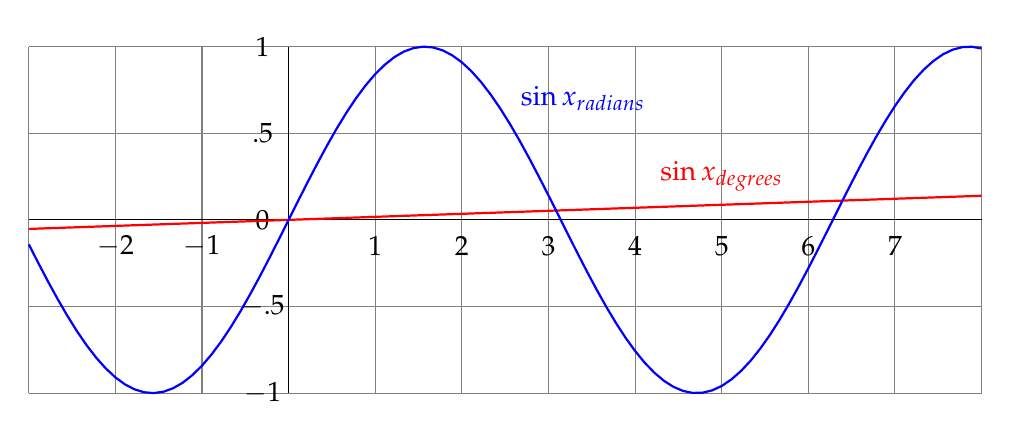
\begin{tikzpicture}[scale=1.1]
\draw[step=10mm,white!50!black,thin] (-3,-2) grid (8,2);
\draw (-3,0) -- (8,0);
\draw (0,-2) -- (0,2);
\foreach \x in {-2,-1,1,2,3,4,5,6,7}
  \node at (\x,-.3) {$\x$};
\foreach \y in {-1,-.5,0,.5,1}
  \node at ($(-.3,0)+(0,2*\y)$) {$\y$};
\draw[red,domain=-3:8,samples=100,thick] plot (\x,{2*sin (\x)});
\draw[blue,domain=-3:8,samples=100,thick] plot (\x,{2*sin (\x r)});
\node[blue] at (3.4,1.4) {$\sin x_{\scriptstyle radians}$};
\node[red] at (5,.5) {$\sin x_{\scriptstyle degrees}$};
\end{tikzpicture}
\caption{The sine function when values in the domain are in radians or degrees}\label{fig.degrees-or-radians}
\end{center}
\end{figure}

\newpage

For the value $1.57$, the value of the sine function depends on the unit of measure, and the difference between radians and degrees is quite large:
\[
\sin\: 1.57_{\scriptstyle radians} \approx 1\,,\;\;\;\;\; \sin \: 1.57_{\scriptstyle degrees}\approx 0.027\,.
\]

Apparently, when we teach trigonometric functions on both degrees and radians, students are unaware of the different representations of the graphs. In practice, students seem to regard the domain of trigonometric function as ``rotations,'' and the units of measurement of the domain of rotations are not important. This leads to inconsistent graphs, where the domain on the $x$-axis is labeled with two different units of measure (Figure~\ref{fig.both-radians-and-degrees}).
 
\begin{figure}[hbt]
\begin{center}
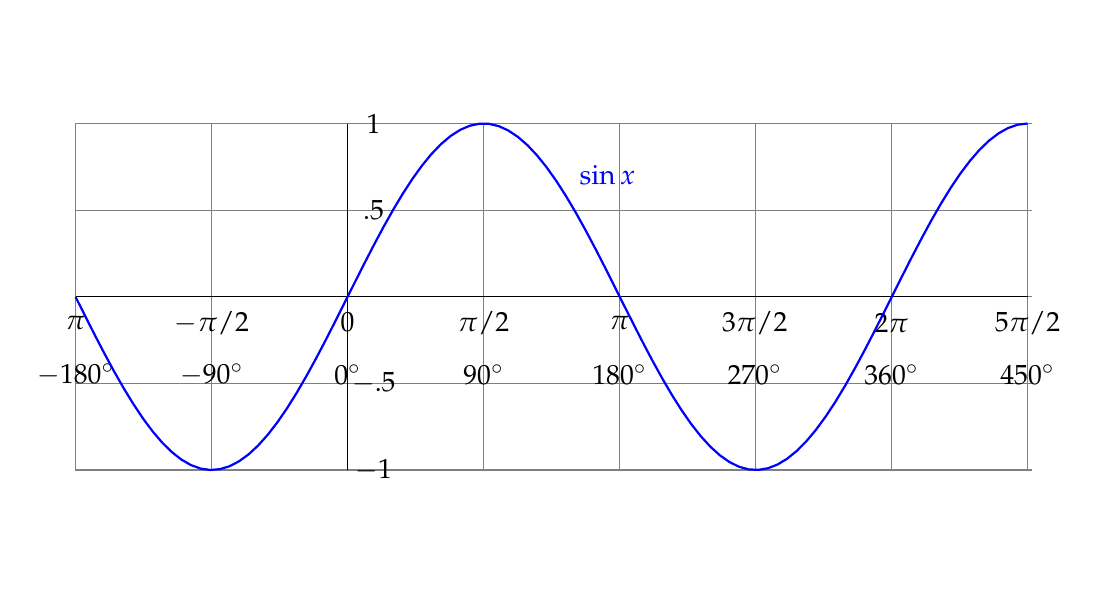
\begin{tikzpicture}[scale=1.1]
\draw[xstep=1.57,ystep=10mm,white!50!black,thin] (-3.15,-2) grid (7.9,2);
\foreach \x/\rad/\deg in {-3.14/\pi/-180^\circ,-1.57/{-\pi/2}/-90^\circ,0/0/0^\circ,1.57/{\pi/2}/90^\circ,3.14/\pi/180^\circ,4.7/{3\pi/2}/270^\circ,6.28/2\pi/360^\circ,7.85/{5\pi/2}/450^\circ} {
  \node at (\x,-.3) {$\rad$};
  \node at (\x,-.9) {$\deg$};
}
\foreach \y/\s in {-3/,-2/-1,-1/-.5,1/.5,2/1,3/} {
  \node at (.3,\y) {$\s$};
}
\draw (-3.14,0) -- (7.85,0);
\draw (0,-2) -- (0,2);
\draw[blue,domain=-3.14:7.85,samples=100,thick] plot (\x,{2*sin (\x r)});
\node[blue] at (3,1.4) {$\sin x$};
\end{tikzpicture}
\caption{Inconsistent units of measures for the same domain}\label{fig.both-radians-and-degrees}
\end{center}
\end{figure}

This dual representation is particularly problematic when discussing the covariance between the values of $x$ and $\sin x$, that is, when studying the derivative of the sine function.
From Figure~\ref{fig.degrees-or-radians} it can seen that \emph{slopes} (and hence the derivatives) of $\sin x_{\scriptstyle \textit{radians}}$ (Figure~\ref{fig.derivative-in-radians}) and $\sin x_{\scriptstyle \textit{degrees}}$ (Figure~\ref{fig.derivative-in-degrees}) are different for equal values of $x$. 

\begin{figure}[htb]
\begin{center}
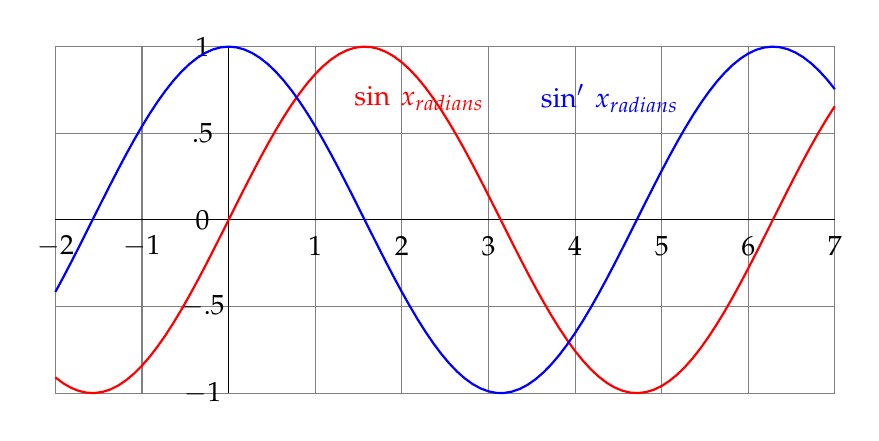
\begin{tikzpicture}[scale=1.1]
\draw[step=10mm,white!50!black,thin] (-2,-2) grid (7,2);
\draw (-2,0) -- (7,0);
\draw (0,-2) -- (0,2);
\foreach \x in {-2,-1,1,2,3,4,5,6,7}
  \node at (\x,-.3) {$\x$};
\foreach \y in {-1,-.5,0,.5,1}
  \node at ($(-.3,0)+(0,2*\y)$) {$\y$};
\draw[red,domain=-2:7,samples=100,thick] plot (\x,{2*sin (\x r)});
\draw[blue,domain=-2:7,samples=100,thick] plot (\x,{2*cos (\x r)});
\node[red] at (2.2,1.4) {$\sin\: x_{\scriptstyle radians}$};
\node[blue] at (4.4,1.4) {$\sin'\: x_{\scriptstyle radians}$};
\end{tikzpicture}
\caption{The sine function and its derivative in radians}\label{fig.derivative-in-radians}
\end{center}
%\end{figure}

%\begin{figure}[htb]
\begin{center}
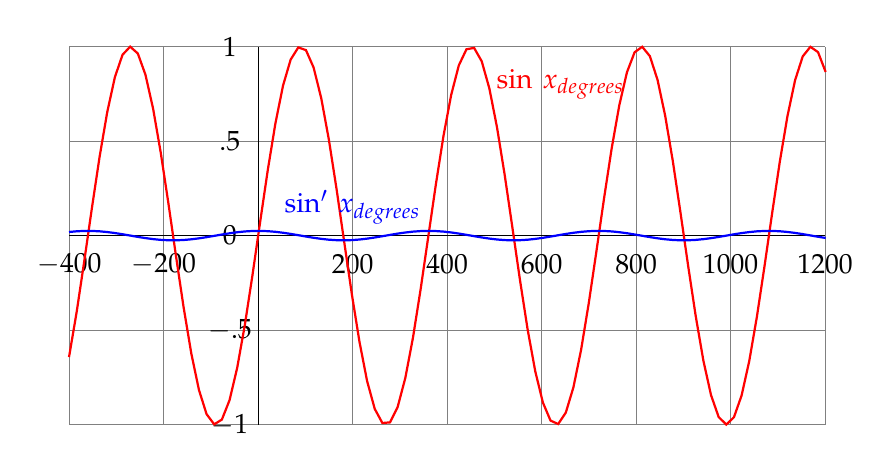
\begin{tikzpicture}[scale=1.2]
\draw[step=10mm,white!50!black,thin] (-2,-2) grid (6,2);
\draw (-2,0) -- (6,0);
\draw (0,-2) -- (0,2);
\foreach \x/\deg in {-2/-400,-1/-200,1/200,2/400,3/600,4/800,5/1000,6/1200}
  \node at (\x,-.3) {$\deg$};
\foreach \y in {-1,-.5,0,.5,1}
  \node at ($(-.3,0)+(0,2*\y)$) {$\y$};
\draw[red,domain=-400:1200,samples=100,thick] plot (0.005*\x,{2*sin (\x)});
\draw[blue,domain=-400:1200,samples=100,thick] plot (0.005*\x,{.05*cos (\x)});
\node[red] at (3.2,1.6) {$\sin\: x_{\scriptstyle degrees}$};
\node[blue] at (1,.3) {$\sin'\: x_{\scriptstyle degrees}$};
\end{tikzpicture}
\caption{The sine function and its derivative in degrees}\label{fig.derivative-in-degrees}
\end{center}
\end{figure}

To understand the graph of $\sin'\: x_{\scriptstyle degrees}$ recall that:
\[
\sin' x=\lim_{h\rightarrow 0} \disfrac{\sin(x+h)-\sin(x)}{h}\,.
\]
For $x=90$ and $h=10$:
\[
\disfrac{\sin(x+h)-\sin(x)}{h} = \disfrac{\sin 100^\circ-\sin 90^\circ}{10}\approx \disfrac{-0.0152}{10}=-0.00152\,,
\]
so we see why the value of $\sin'\: x_{\scriptstyle degrees}$ is very small.

We must choose one of the two representations.
From Figures~\ref{fig.derivative-in-radians},~\ref{fig.derivative-in-degrees}, we can see that the derivative of $\sin'\: x_{\scriptstyle radians}$ is $\cos\: x_{\scriptstyle radians}$ while the derivative of $\sin'\: x_{\scriptstyle degrees}$ is $a\cdot\cos x_{\scriptstyle degrees}$ where $a\ll 1$.
We can justify the choice of defining the trigonometric functions on a domain measured in radians for reasons of mere convenience.
Of course, there are other considerations for selecting radians and these will be discussed below.

\section{Periodic functions: the winding operation}

Trigonometric functions are \emph{periodic}.
While it is possible to discuss periodic functions initially in the context of trigonometry, we suggest that the topic be discussed earlier.\footnote{The following activity was shown to us by Zippora Resnick.}

\begin{wrapfigure}[11]{r}{.5\textwidth}
%\begin{figure}[hbt]
\begin{center}
\vspace{-6ex}
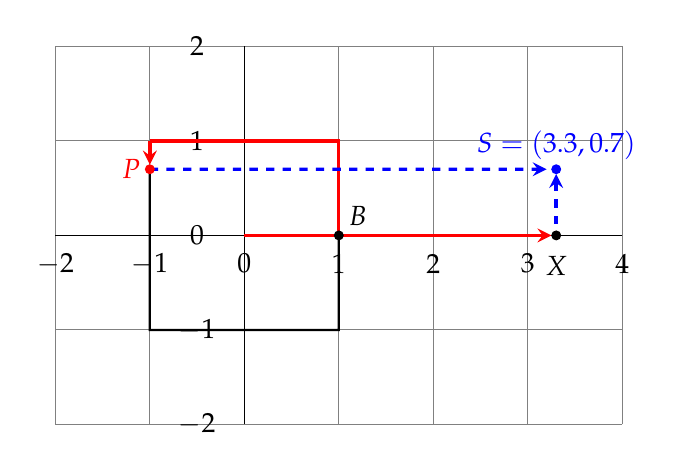
\begin{tikzpicture}[scale=1.2]
\draw[step=10mm,white!50!black,thin] (-2,-2) grid (4,2);
\draw (-2,0) -- (4,0);
\draw (0,-2) -- (0,2);
\foreach \x in {-2,-1,0,1,2,3,4}
  \node at (\x,-.3) {$\x$};
\foreach \y in {-2,-1,0,1,2}
  \node at ($(-.5,0)+(0,\y)$) {$\y$};
\coordinate (X) at (3.3,0);
\draw[red,very thick,->] (0,0) -- (3.25,0);
\draw[red,very thick] (1,0) -- (1,1) -- (-1,1);
\coordinate (P) at (-1,.7);
\draw[red,very thick,->] (-1,1) -- (-1,.75);
\draw[thick] (P) -- (-1,-1) -- (1,-1) -- (1,0);
\coordinate (S) at (3.3,0.7);
\draw[blue,very thick,dashed,->] (P) -- (3.2,0.7);
\draw[blue,very thick,dashed,<-] (3.3,.65) -- (3.3,0);
\fill[blue] (S) circle(1.5pt) node[above] {$S=(3.3,0.7)$};
\fill (X) circle(1.5pt) node[below,yshift=-4pt] {$X$};
\fill (1,0) circle(1.5pt) node[above right] {$B$};
\fill[red] (P) circle(1.5pt) node[left] {$P$};
\end{tikzpicture}
\caption{Winding a thread around a square}\label{fig.winding-around-a-square}
\end{center}
%\end{figure}
\end{wrapfigure}

We construct a function that maps real numbers to real numbers, where the domain is the set of lengths obtained by winding a thread (real or imaginary) around a geometric shape, \emph{not necessarily a circle}.
Consider a square centered at the origin of the coordinate system, oriented so that its its sides are parallel to the axes and the length of each side is two units (Figure~\ref{fig.winding-around-a-square}).
For any given value of $x$, take a thread of length $|x|$ and wind it around the square starting $(1,0)$. As usual the thread is wound counterclockwise $x>0$ and clockwise if $x <0$.
Label the point on the square reached at the end of the thread by $P$.


Let us construct the function that maps of the length of the thread $x$ to the $y$ coordinate of $P$. In the Figure, we see that $x=3.3$ is mapped into $y=0.7$.
This function is periodic with a period equal to the perimeter of the square: $f(x+8k)=f(x), k\in \mathcal{Z}$.

A fruitful exercise for students is to explore the winding operation for various polygons (\geoproject{g.winding}).


\begin{itemize}
\item \url{https://www.geogebra.org/m/QRmStjFg} is another project on periodic functions.
\item \url{https://scratch.mit.edu/studios/25046732} is a collection of programs in Scratch that demonstrate winding around a circle.
\end{itemize}


\section{The function \texorpdfstring{$s$}{s} maps a real number to a coordinate}

In the previous section, we defined a function by winding a thread around a polygon. As the number of sides of a (regular) polygon increases, the polygon converges to a circle. The trigonometric functions are defined by winding around a unit circle: a circle of radius $1$ centered at $(0,0)$. The beginning of the thread is at $(1,0)$. The functions will be periodic with period the ``perimeter'' (circumference) of the circle, $2\pi$.

Figure~\ref{fig.winding-around-a-square} shows a correlation between two points, $P$ on the perimeter of the polygon and $S$, the point defined by the intersection of a horizontal line through $P$ and a vertical line through $X$.
However, a function is defined as a mapping between a value in its domain to a value in its range, not as a correlation between two points, each with an $x$ and $y$ value.
Therefore, we define a function $s(x)$ that maps the $x$ value of $S$ and $X$ (only) to the $y$ value of $P$ and $S$.

Of course, teachers immediately see that $s$ is the sine function, but they must consider if they wish to point this out to the students.
In the functional approach, it makes sense to defer discussing the relationship with trigonometric functions defined in right triangles, which the students possibly know from previous study of mathematics and physics.
The reason is that the concept of a function as a mapping from all real numbers to points on the unit circle should be firmly established before making the transition to the triangular definitions.

\begin{figure}[hbt]
\begin{center}
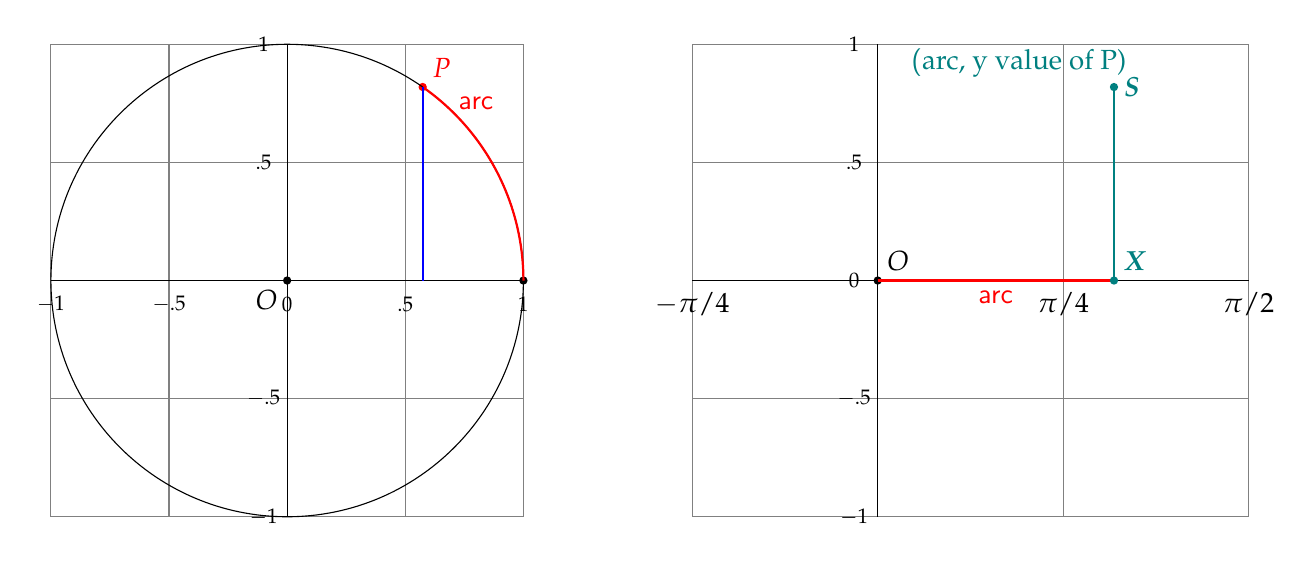
\begin{tikzpicture}[scale=1.5]
\begin{scope}
\draw[step=10mm,white!50!black,thin] (-2,-2) grid (2,2);
\draw (-2,0) -- (2,0);
\draw (0,-2) -- (0,2);
\foreach \x in {-1,-.5,0,.5,1}
  \node at (2*\x,-.2) {$\scriptstyle \x$};
\foreach \y in {-1,-.5,.5,1}
  \node at ($(-.2,0)+(0,2*\y)$) {$\scriptstyle \y$};
\coordinate (O) at (0,0);
\coordinate (B) at (2,0);
\coordinate (P) at (55:2);
\fill (O) circle(1pt) node [below left] {$O$};
\fill (B) circle(1pt);
\fill[red] (P) circle(1pt) node [above right] {$P$};
\node[draw, name path = circle] at (O)
    [circle through = (P)] {};
\draw[red,thick] (B) arc[start angle=0,end angle=55,radius=2cm];
\node[red] at (1.6,1.5) {$\textsf{arc}$};
\draw[blue,thick] (P) -- (P |- O);
\end{scope}
\begin{scope}[xshift=5cm]
\draw[xstep=1.57,ystep=10mm,white!50!black,thin] (-1.57,-2) grid (3.14,2);
\draw (-1.57,0) -- (3.14,0);
\draw (0,-2) -- (0,2);
\foreach \x/\tick in {-1.57/{-\pi/4},1.57/{\pi/4},3.14/{\pi/2}}
  \node at (\x,-.2) {$\tick$};
\foreach \y in {-1,-.5,0,.5,1}
  \node at ($(-.2,0)+(0,2*\y)$) {$\scriptstyle \y$};
\coordinate (O) at (0,0);
\coordinate (B) at (2,0);
\fill (O) circle(1pt) node [above right] {$O$};
\coordinate (S) at (1*2,.819*2);
\fill[teal] (S) circle(1pt)
  node [above left,xshift=8pt] {\textsf(arc,\ y value of P)}
  node[right,teal] {$\bm{S}$};
\draw [thick,teal] (S) -- (S |- O) coordinate (X);
\draw[thick,red] (O) -- node[below] {\textsf{arc}} (X);
\fill[teal] (X) circle(1pt) node[above right] {$\bm{X}$};
\end{scope}
\end{tikzpicture}
%\includegraphics[width=\textwidth,keepaspectratio]{sine-radians-split}
\caption{Definition of the function $s(x)$}\label{fig.function-s}
\end{center}
\end{figure}

Figure~\ref{fig.function-s} (\geoproject{g.sine}) shows the definition of the function $s(x)$ in a split window: the right window shows the independent variable (point $X$) and the dependent variable (point $S$), which is the value of the function . The left window shows the geometric construction that defines the function.\footnote{In Geogebra, constructions such as these can be done in a single screen (\geoproject{g.single}) or in a split screen (\geoproject{g.split}).}
The $x$-value of $X$, the independent variable, is used as the length of an arc from point $(1,0)$ around the circumference of the unit circle.
The $y$-value of $P$, the dependent variable, is the length of a perpendicular line from $P$ to the $x$-axis.


%\begin{figure}[hbt]
\begin{wrapfigure}[8]{r}{.6\textwidth}
\begin{center}
\vspace{-5ex}
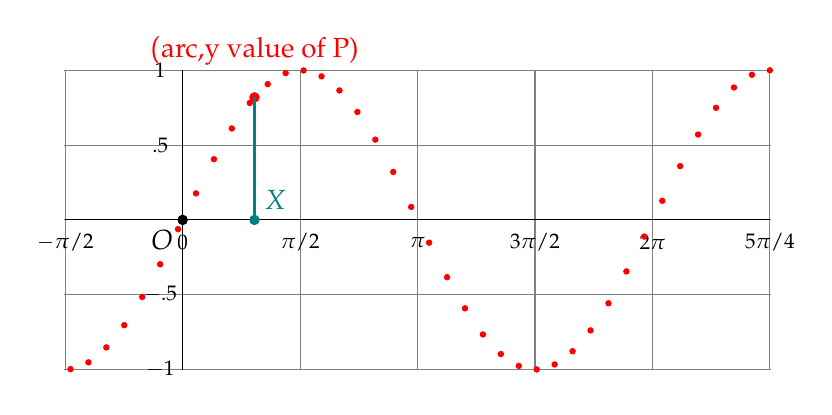
\begin{tikzpicture}[scale=.95]
\draw[xstep=1.57cm,ystep=1cm,white!50!black,thin]
  (-1.58,-2) grid (7.86,2);
\draw (-1.57,0) -- (7.85,0);
\draw (0,-2) -- (0,2);
\foreach \x/\tick in {-1.57/{-\pi/2},0/0,1.57/{\pi/2},3.14/{\pi},4.71/{3\pi/2},6.28/{2\pi},7.85/{5\pi/4}}
  \node at (\x,-.3) {$\scriptstyle \tick$};
\foreach \y in {-1,-.5,.5,1}
  \node at ($(-.3,0)+(0,2*\y)$) {$\scriptstyle \y$};
\path[red,domain=-1.5:7.85,samples=40,mark=*,mark size=1pt] plot (\x,{2*sin (\x r)});
\coordinate (P) at (.960,.819*2);
\coordinate (O) at (0,0);
\fill (O) circle(2pt) node [below left] {$O$};
\fill[red] (P) circle(2pt) node [above,yshift=8pt] {\textsf(arc,y value of P)};
\draw [very thick,teal] (P) -- (P |- O) coordinate (X);
\fill[teal] (X) circle(2pt) node[above right] {$X$};
\end{tikzpicture}
%\includegraphics[width=\textwidth,keepaspectratio]{trace-of-the-function}
\caption{Trace of the function $s$}\label{fig.trace-of-the-function}
\end{center}
%\end{figure}
\end{wrapfigure}

The graphical representation of the function for all real values can be obtained by tracing the points $P$ as you drag the point $X$ left and right (Figure~\ref{fig.trace-of-the-function}, \geoproject{g.trace})

The graphical representation reveals the periodicity of the function: $s(x) = s(x + 2\pi k), k\in \mathcal{Z}$.

\section{Symmetries of the function \texorpdfstring{$s$}{s}}

When winding around a circle (as when winding around a square), by symmetry there are close relationships between values of the functions for points $P$ located in the four quadrants.
Clearly, for every point $P_1$ in the first quadrant there is a point $P_2$ in the second quadrant with $x_2=-x_1$ and $y_2=y_1$.
These relationships can be explored by the students even before the trigonometric functions are defined.

Figure~\ref{fig.symmetries} (left) displays points obtained by reflections of the point $P$ which is the endpoint of the arc starting from $(1,0)$. The following table lists the points obtained by reflection:
\begin{center}
\begin{tabular}{|l|l|}
\hline
$P$ & Endpoint of the arc\\\hline
$P_x$ & Reflection around the $x$-axis\\\hline
$P_y$ & Reflection around the $y$-axis\\\hline
$P_{xy}$ & Reflection around the origin\\\hline
\end{tabular}
\end{center}

\bigskip

\begin{figure}[hbt]
\begin{minipage}{.45\textwidth}
\begin{center}
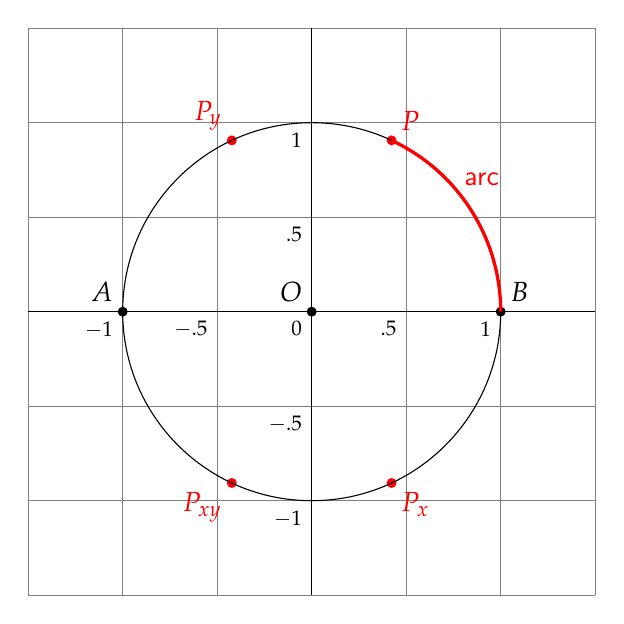
\begin{tikzpicture}[scale=1.2]
\draw[step=10mm,white!50!black,thin] (-3,-3) grid (3,3);
\draw[thin] (-3,0) -- (3,0);
\draw[thin] (0,-3) -- (0,3);
  \coordinate[label = above left:$A$]  (A) at (-2,0);
  \coordinate[label = above right:$B$] (B) at (2,0);
  \coordinate[label = above left:$O$] (O) at (0,0);
%  \coordinate[label = above right:$H$] (H) at (0,2);
%  \coordinate[label = below right:$G$] (G) at (0,-2);
  \fill (A) circle (1.5pt);
  \fill (B) circle (1.5pt);
  \fill (O) circle (1.5pt);
%  \fill (H) circle (1.5pt);
%  \fill (G) circle (1.5pt);
  \coordinate (P) at (65:2);
  \coordinate (Py) at (115:2);
  \coordinate (Pxy) at (-115:2);
  \coordinate (Px) at (-65:2);
  \fill[red] (P) circle (1.5pt) node[above right] {$P$};
  \fill[red] (Pxy) circle (1.5pt) node[below left] {$P_{xy}$};
  \fill[red] (Py) circle (1.5pt) node[above left] {$P_y$};
  \fill[red] (Px) circle (1.5pt) node[below right] {$P_x$};
\foreach \x/\tick in {-2/-1,-1/-.5,0/0,1/.5,2/1}
  \node[below left] at (\x,0) {$\scriptstyle\tick$};
\foreach \y/\tick in {-2/-1,-1/-.5,1/.5,2/1}
  \node[below left] at (0,\y) {$\scriptstyle\tick$};
  \node[draw, name path = circle] at (O)
    [circle through = (A)] {};
\draw[red,very thick] (B) arc[start angle=0,end angle=65,radius=2cm];
\node[red] at (1.8,1.4) {\textsf{arc}};
\end{tikzpicture}
\end{center}
\end{minipage}
\hspace{2em}
\begin{minipage}{.45\textwidth}
\begin{center}
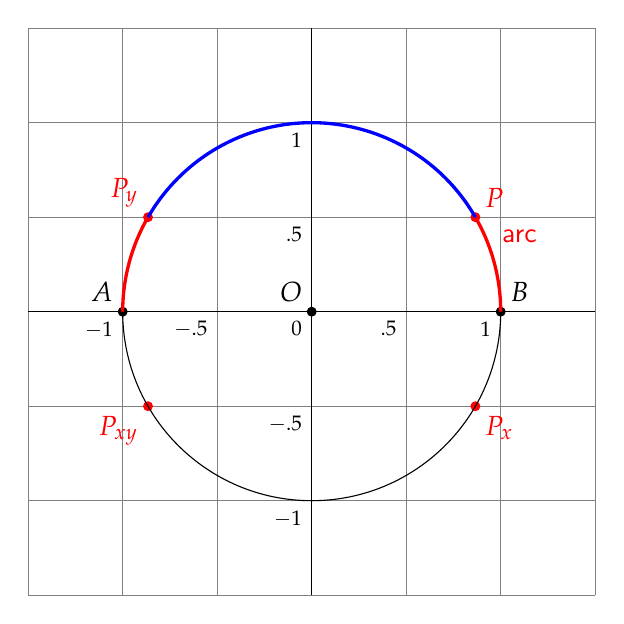
\begin{tikzpicture}[scale=1.2]
\draw[step=10mm,white!50!black,thin] (-3,-3) grid (3,3);
\draw[thin] (-3,0) -- (3,0);
\draw[thin] (0,-3) -- (0,3);
  \coordinate[label = above left:$A$]  (A) at (-2,0);
  \coordinate[label = above right:$B$] (B) at (2,0);
  \coordinate[label = above left:$O$] (O) at (0,0);
%  \coordinate[label = above right:$H$] (H) at (0,2);
%  \coordinate[label = above right:$G$] (G) at (0,-2);
  \fill (A) circle (1.5pt);
  \fill (B) circle (1.5pt);
  \fill (O) circle (1.5pt);
%  \fill (H) circle (1.5pt);
%  \fill (G) circle (1.5pt);
  \coordinate (P) at (30:2);
  \coordinate (Py) at (150:2);
  \coordinate (Pxy) at (-150:2);
  \coordinate (Px) at (-30:2);
  \fill[red] (P) circle (1.5pt) node[above right] {$P$};
  \fill[red] (Pxy) circle (1.5pt) node[below left] {$P_{xy}$};
  \fill[red] (Py) circle (1.5pt) node[above left] {$P_y$};
  \fill[red] (Px) circle (1.5pt) node[below right] {$P_x$};
\foreach \x/\tick in {-2/-1,-1/-.5,0/0,1/.5,2/1}
  \node[below left] at (\x,0) {$\scriptstyle\tick$};
\foreach \y/\tick in {-2/-1,-1/-.5,1/.5,2/1}
  \node[below left] at (0,\y) {$\scriptstyle\tick$};
  \node[draw, name path = circle] at (O)
    [circle through = (A)] {};
\draw[red,very thick] (B) arc[start angle=0,end angle=30,radius=2cm];
\draw[red,very thick] (A) arc[start angle=180,end angle=150,radius=2cm];
\draw[blue,very thick] (P) arc[start angle=30,end angle=150,radius=2cm];
\node[red] at (2.2,.8) {\textsf{arc}};
\end{tikzpicture}
\end{center}
\end{minipage}
\caption{Symmetries of the function $s$}\label{fig.symmetries}
\end{figure}


By examining the Figure we conclude that:
\begin{eqnarray*}
s(P_x) &=& -s(P)\\
s(P_y) &=& s(P)\\
s(P_{xy}) &=& -s(P)\,.
\end{eqnarray*}

Consider now Figure~\ref{fig.symmetries} (right). Since $P_y$ is the reflection of $P$ about the $y$ axis, the length of the arc from $A$ to $P_y$ is the same as the length of the arc from $B$ to $P$. Therefore, if the length of the arc from $A$ to $P_y$ is $x$, the length of the arc from $B$ to $P_y$ is $\pi-x$, so we conclude that:
\[
s(x) = s(\pi - x)\,.
\]
Since $P$ was chosen arbitrarily, this is true for any $x$.

Additional symmetries can be derived in the same way:
\begin{eqnarray*}
s(x) &=& -s(-x)\\
s(\pi+x) &=& -s(x)\\
s(\pi-x) &=& s(x)\,.
\end{eqnarray*}
From $s(x) = -s(-x)$ it follows that the function is odd.

The cyclic and symmetrical properties facilitate obtaining values of the function $s$. This of great help to students since they need remember only a few values of $s$.

\newpage

%\begin{figure}[hbt]
\begin{wrapfigure}[12]{r}{.6\textwidth}
\begin{center}
\vspace{-2ex}
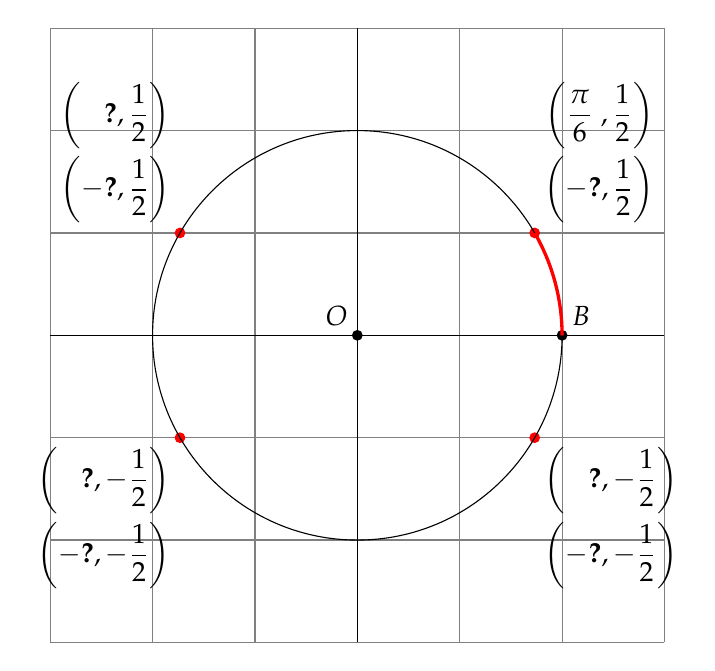
\begin{tikzpicture}[scale=1.3]
  \draw[step=10mm,white!50!black,thin] (-3,-3) grid (3,3);
  \draw[thin] (-3,0) -- (3,0);
  \draw[thin] (0,-3) -- (0,3);
  \coordinate[label = above right:$B$] (B) at (2,0);
  \coordinate[label = above left:$O$] (O) at (0,0);
  \fill (B) circle (1.5pt);
  \fill (O) circle (1.5pt);
  \coordinate (P) at (30:2);
  \coordinate (Py) at (150:2);
  \coordinate (Pxy) at (-150:2);
  \coordinate (Px) at (-30:2);
  \fill[red] (P) circle (1.5pt) node[black,above right]
     {
      \shortstack{
         $\left(\disfrac{\pi}{6}\;,
             \disfrac{1}{2}\right)$
      \\
      $\left(-\bm{?},
             \disfrac{1}{2}\right)$}};
  \fill[red] (Pxy) circle (1.5pt) node[below left,black]
     {
      \shortstack{
         $\left(\;\;\;\bm{?},
             -\disfrac{1}{2}\right)$
      \\
      $\left(-\bm{?},
             -\disfrac{1}{2}\right)$}};
  \fill[red] (Py) circle (1.5pt) node[above left,black]
     {
      \shortstack{
         $\left(\;\;\;\bm{?},
             \disfrac{1}{2}\right)$
      \\
      $\left(-\bm{?},
             \disfrac{1}{2}\right)$}};
  \fill[red] (Px) circle (1.5pt) node[below right,black]
     {
      \shortstack{
         $\left(\;\;\;\bm{?},
             -\disfrac{1}{2}\right)$
      \\
      $\left(-\bm{?},
             -\disfrac{1}{2}\right)$}};
  \node[draw, name path = circle] at (O)
    [circle through = (B)] {};
  \draw[red,very thick] (B)
     arc[start angle=0,end angle=30,radius=2cm];
\end{tikzpicture}
\caption{Computing values of the function $s$}\label{fig.computing}
\end{center}
%\end{figure}
\end{wrapfigure}

A good exercise at this point is to identify the values $V=\{x_1,x_2,\ldots\}$ of $x$ that such that $s(x_i)=\pm s(x)$. Suppose we know that $s(\pi/6)=1/2$. We now ask for the value of $x$ for the three symmetrical points (Figure~\ref{fig.computing}). Each point is also reached by winding the thread around the circle in a negative direction. Finally, since the function is periodic, for example, $s(-5\pi/6)=1/2$, $V=\{x_1,x_2,\ldots\}$ is an infinite set.

\vspace{10ex}

\section{The function \texorpdfstring{$c$}{c} maps a real number to a coordinate}

The definition of the function $s$ leads naturally to the definition of a function $c$ which maps a real number (the length of an arc on the circumference of the unit circle) to the $x$-value of the end point of the arc (Figure~\ref{fig.cosine}, \geoproject{g.cosine}).
\begin{figure}[H]
\begin{center}
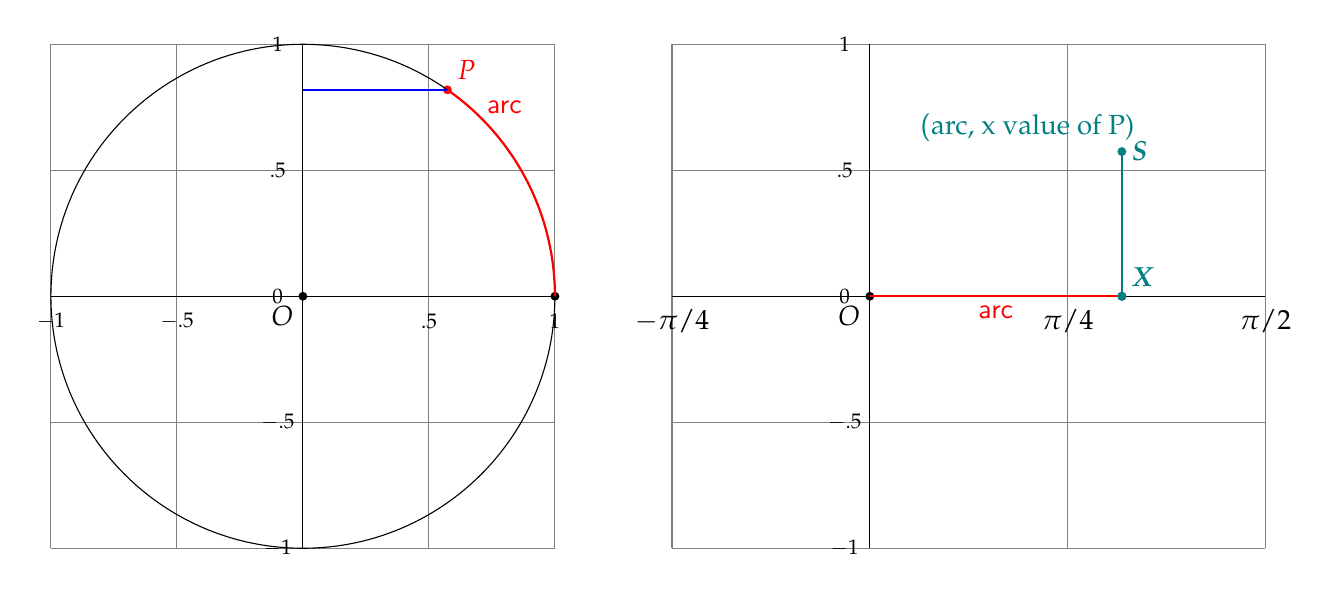
\begin{tikzpicture}[scale=1.6]
\begin{scope}
\draw[step=10mm,white!50!black,thin] (-2,-2) grid (2,2);
\draw (-2,0) -- (2,0);
\draw (0,-2) -- (0,2);
\foreach \x in {-1,-.5,.5,1}
  \node at (2*\x,-.2) {$\scriptstyle \x$};
\foreach \y in {-1,-.5,0,.5,1}
  \node at ($(-.2,0)+(0,2*\y)$) {$\scriptstyle \y$};
\coordinate (O) at (0,0);
\coordinate (B) at (2,0);
\coordinate (P) at (55:2);
\fill (O) circle(1pt) node [below left] {$O$};
\fill (B) circle(1pt);
\fill[red] (P) circle(1pt) node [above right] {$P$};
\node[draw, name path = circle] at (O)
    [circle through = (P)] {};
\draw[red,thick] (B) arc[start angle=0,end angle=55,radius=2cm];
\node[red] at (1.6,1.5) {$\textsf{arc}$};
\draw[blue,thick] (P) -- (P -| O);
\end{scope}
\begin{scope}[xshift=4.5cm]
\draw[xstep=1.57,ystep=10mm,white!50!black,thin] (-1.57,-2) grid (3.14,2);
\draw (-1.57,0) -- (3.14,0);
\draw (0,-2) -- (0,2);
\foreach \x/\tick in {-1.57/{-\pi/4},1.57/{\pi/4},3.14/{\pi/2}}
  \node at (\x,-.2) {$\tick$};
\foreach \y in {-1,-.5,0,.5,1}
  \node at ($(-.2,0)+(0,2*\y)$) {$\scriptstyle \y$};
\coordinate (O) at (0,0);
\coordinate (B) at (2,0);
%\coordinate (P) at (.960*2,.574*2);
\coordinate (S) at (1*2,.574*2);
\fill (O) circle(1pt) node [below left] {$O$};
\fill (B) circle(1pt);
\fill[teal] (S) circle(1pt) node [teal,above left,xshift=8pt]
   {\textsf(arc,\ x value of P)}
   node[right,teal] {$\bm{S}$};
\draw [thick,teal] (S) -- (S |- O) coordinate (X);
\draw[thick,red] (O) -- node[below] {\textsf{arc}} (X);
\fill[teal] (X) circle(1pt) node[above right] {$\bm{X}$};
\end{scope}
\end{tikzpicture}
%\includegraphics[width=\textwidth,keepaspectratio]{sine-radians-split}
\caption{Geometric construction that defines the function $c(x)$}\label{fig.cosine}
\end{center}
\end{figure}

Be careful: the notation may lead to confusion.
The \emph{point} $X$ (upper case) identifies a point along the $x$-axis. The length from the origin to $X$ specifies the length of the arc from $(1,0)$ around the circumference of the circle.
The \emph{variable} $x$ (lower case) is the $x$ value of the coordinates of $P$, the endpoint of this arc.

In the Geogebra project, a trace of the value of $c(x)$ as $x$ is moved along the $x$-axis gives a graphical representation of the function (Figure~\ref{fig.cosine-trace}).

\begin{figure}[hbt]
\begin{center}
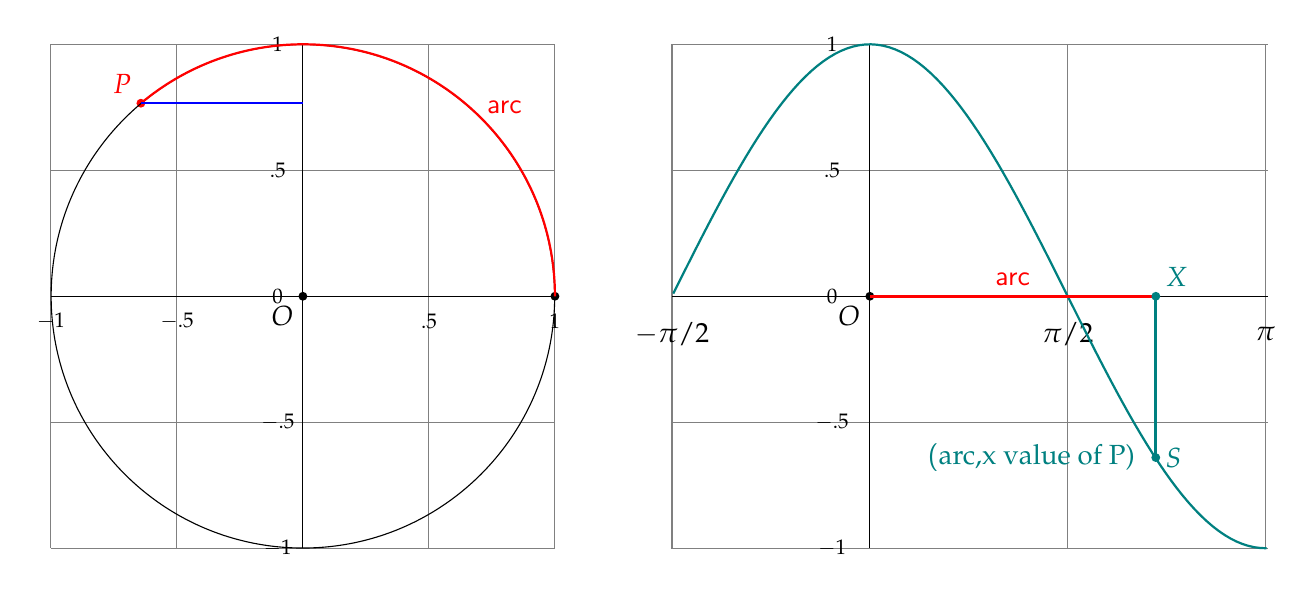
\begin{tikzpicture}[scale=1.6]
\begin{scope}
\draw[step=10mm,white!50!black,thin] (-2,-2) grid (2,2);
\draw (-2,0) -- (2,0);
\draw (0,-2) -- (0,2);
\foreach \x in {-1,-.5,.5,1}
  \node at (2*\x,-.2) {$\scriptstyle \x$};
\foreach \y in {-1,-.5,0,.5,1}
  \node at ($(-.2,0)+(0,2*\y)$) {$\scriptstyle \y$};
\coordinate (O) at (0,0);
\coordinate (B) at (2,0);
\coordinate (P) at (130:2);
\fill (O) circle(1pt) node [below left] {$O$};
\fill (B) circle(1pt);
\fill[red] (P) circle(1pt) node [above left] {$P$};
\node[draw, name path = circle] at (O)
    [circle through = (P)] {};
\draw[red,thick] (B) arc[start angle=0,end angle=130,radius=2cm];
\node[red] at (1.6,1.5) {$\textsf{arc}$};
\draw[blue,thick] (P) -- (P -| O);
\end{scope}
\begin{scope}[xshift=4.5cm]
\draw[xstep=1.57cm,ystep=1cm,white!50!black,thin] (-1.58,-2) grid (3.16,2);
\draw (-1.57,0) -- (3.16,0);
\draw (0,-2) -- (0,2);
\foreach \x/\tick in {-1.57/{-\pi/2},1.57/{\pi/2},3.14/{\pi}}
  \node at (\x,-.3) {$\tick$};
\foreach \y in {-1,-.5,0,.5,1}
  \node at ($(-.3,0)+(0,2*\y)$) {$\scriptstyle\y$};
\draw[thick,teal,domain=-1.56:3.15,samples=100] plot (\x,{2*cos (\x r)});
\coordinate (S) at (2.269,-.64*2);
\coordinate (O) at (0,0);
\fill (O) circle(1pt) node [below left] {$O$};
\fill[teal] (S) circle(1pt) node [right] {$S$}
  node[left,xshift=-4pt] {\textsf(arc,x value of P)};
\draw [very thick,teal] (S) -- (S |- O) coordinate (X);
\draw[very thick,red] (O) -- node[above] {\textsf{arc}} (X);
\fill[teal] (X) circle(1pt) node[above right] {$X$};
\end{scope}
\end{tikzpicture}
%\includegraphics[width=\textwidth,keepaspectratio]{sine-radians-split}
\caption{Trace of the function $c(x)$}\label{fig.cosine-trace}
\end{center}
\end{figure}

From Figures~\ref{fig.symmetries}, symmetry properties of $c(x)$ can be derived. We leave it to the reader to justify the following equalities:
\begin{eqnarray*}
c(P_x) &=& c(P)\\
c(P_y) &=& -c(P)\\
c(P_{xy}) &=& -c(P)\,.
\\
c(x) &=& -c(\pi - x)\\
c(x) &=& c(-x)\\
c(\pi+x) &=& -c(x)\\
c(\pi-x) &=& -c(x)\,.
\end{eqnarray*}
Figure~\ref{fig.computing} can be modified to ask questions about the function $c(x)$.

At this point, the teacher faces the dilemma whether to continue the study of the sine and cosine functions (specifically, translation and change of radius) or the move on the tangential trigonometric functions.
Both choices are legitimate.
There is a significant advantage to continuing with the trigonometric functions already presented. 
This can firmly establish the concept that trigonometric functions are true functions that can be modified by performing arithmetic operations of the domain values or on the range values.
Once this has been done, the tangential functions can be taught.

Translation and change of radius is discussed in a separate Chapter~\ref{ch.translated}.



\section{Tangential trigonometric functions}

The standard approach is to define the tangent function as a correlation between a real number (that defines the length and direction of an arc) and the $y$ value of the intersection of (1) the line passing through the center of the coordinate system and the endpoint of the arc $P$, and (2) a vertical line tangent to the unit circle at $(1,0)$ (Figure~\ref{fig.tangent}, \geoproject{g.tangent}).

\begin{figure}[hbt]
\begin{center}
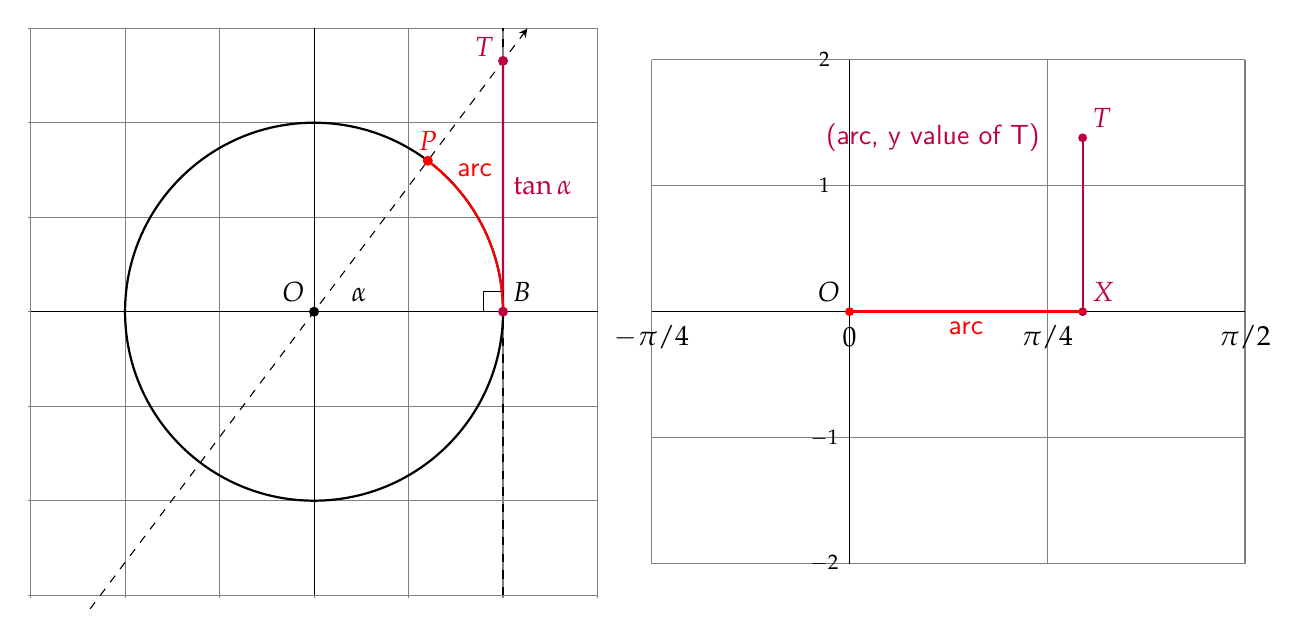
\begin{tikzpicture}
\begin{scope}[scale=.6]
\draw[step=2cm,white!50!black,thin] (-6.05,-6.05) grid (6,6);
\draw[thin] (-6,0) -- (6,0);
\draw[thin] (0,-6) -- (0,6);
  \coordinate (A) at (-4,0);
  \coordinate[label = above right:$B$] (B) at (4,0);
  \coordinate[label = above left:$O$] (O) at (0,0);
  \draw (O) -- (6,0);
  \node[draw, thick, name path = circle] at (O)
    [circle through = (A)] {};
  \coordinate (TT) at (53:7.5);
  \draw[dashed,name path=side,->] ($(O)!-1.05!(TT)$) -- (TT);
  \draw[name path=tangent,dashed] (4,-6) -- (4,6);
  \path [name intersections = {of = circle and side, by = {C}}];
  \path [name intersections = {of = side and tangent, by = {T}}];
  \draw[thick,purple] (B) -- node[right] {$\tan\alpha$} (T);
  \draw[rotate=90] (B) rectangle +(12pt,12pt);
  \draw[thick,red] (B) arc [start angle = 0, end angle = 53, radius=4];
  \node[red] at (3.4,3) {\textsf{arc}};
  \fill[red] (C) circle (3pt) node[above] {$P$};
  \fill[purple] (T) circle (3pt) node[above left,yshift=-2pt] {$T$};
  \fill (O) circle (3pt) node[above right,xshift=10pt] {$\alpha$};
  \fill[purple] (B) circle (3pt);
\end{scope}
\begin{scope}[xshift=6.8cm,scale=1.6]
\draw[xstep=1.57,ystep=1,white!50!black,thin] (-1.57,-2) grid (3.14,2);
\draw (-1.57,0) -- (3.14,0);
\draw (0,-2) -- (0,2);
\foreach \x/\tick in {-1.57/{-\pi/4},0,1.57/{\pi/4},3.14/{\pi/2}}
  \node at (\x,-.2) {$\tick$};
\foreach \y/\tick in {-1/-2,-.5/-1,.5/1,1/2}
  \node at ($(-.2,0)+(0,2*\y)$) {$\scriptstyle \tick$};
\coordinate (O) at (0,0);
\coordinate (Tan) at (.925*2,1.38);
\fill[red] (O) circle(1pt) node [above left,black] {$O$};
\fill[purple] (Tan) circle(1pt) node [above right] {$T$} node[left,xshift=-12pt] {\textsf{(arc, y value of T)}};
\draw[thick,purple] (Tan) -- (Tan |- O) coordinate (X);
\fill[purple] (X) circle(1pt) node[above right] {$X$};
\draw[very thick,red] (O) -- node[below] {\textsf{arc}} (X);
\end{scope}
\end{tikzpicture}
%\includegraphics[width=\textwidth,keepaspectratio]{tangent}
\caption{The tangent function}\label{fig.tangent}
\end{center}
\end{figure}

This definition is consistent with the triangular definition. In the triangle $\triangle TBO$, $\tan \alpha$ is opposite $TB$ over adjacent $OB$ which is $1$ in the unit circle.

The tangent function demonstrates a periodic function with period $\pi$, but it is undefined for an infinite number of real values. This can be seen geometrically: as $\alpha$ approaches $\disfrac{\pi}{2}+\pi k, k in \mathcal{Z}$, the line $OP$ approaches a line parallel to the line $x=1$. The $y$-coordinate of the intersection $T$ becomes larger and larger, approaching infinity.

Conversely, for an arc whose length is any real number $a$, find the point $T=(1,a)$. $TB$ is the tangent of the angle of the line through the intersection of $O$ and $T$ relative to the $x$-axis.
This demonstrates that the tangent function tangent can take any real value.

Similarly, the cotangent function is defined as the intersection of the line through $O$ and $P$ with the horizontal line $y = 1$ (Figure~\ref{fig.cotangent}, \geoproject{g.cotangent}).

This definition is consistent with the triangular definition. In the congruent triangles $\triangle CDO,\triangle C'EO$, $\cot \alpha$ is adjacent $CD$ over opposite $OD$ which is $1$ in the unit circle. Since both the sine and cosine of $\angle BOP$ are the negatives of those of $\angle BOC$, their quotient is positive.


\begin{figure}[hbt]
\begin{center}
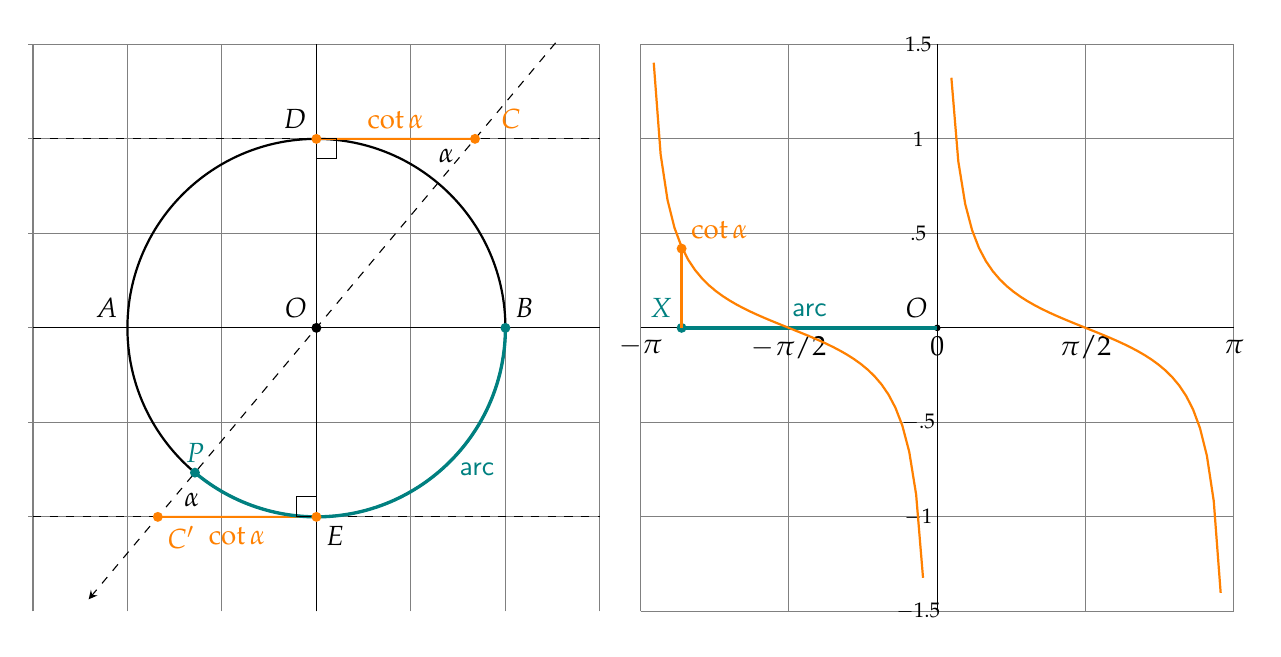
\begin{tikzpicture}
\begin{scope}[scale=.6]
\draw[step=2cm,white!50!black,thin] (-6.1,-6) grid (6,6);
\draw[thin] (-6,0) -- (6,0);
\draw[thin] (0,-6) -- (0,6);
  \coordinate[label = above left:$A$] (A) at (-4,0);
  \coordinate[label = above right:$B$] (B) at (4,0);
  \coordinate[label = above left:$D$] (D) at (0,4);
  \coordinate[label = below right:$E$] (E) at (0,-4);
  \coordinate[label = above left:$O$] (O) at (0,0);
  \draw (O) -- (6,0);
  \node[draw, thick, name path = circle] at (O)
    [circle through = (A)] {};
  \coordinate (TT) at (-130:7.5);
  \draw[dashed,name path=side,->] ($(O)!-1.05!(TT)$) -- (TT);
  \draw[name path=cotangent,dashed] (-6,4) -- (6,4);
  \draw[name path=cotangent-prime,dashed] (-6,-4) -- (6,-4);
  \path [name intersections = {of = side and cotangent, by = {C}}];
  \path [name intersections = {of = side and cotangent-prime, by = {Cprime}}];
  \draw[thick,orange] (D) -- node[above] {$\cot\alpha$} (C);
  \draw[thick,orange] (E) -- node[below] {$\cot\alpha$} (Cprime);
  \draw[very thick,teal] (B) arc [start angle = 0, end angle = -130, radius=4];
  \node[teal] at (3.4,-3) {\textsf{arc}};
  \draw[rotate=-90] (D) rectangle +(12pt,12pt);
  \draw[rotate=90] (E) rectangle +(12pt,12pt);
  \fill[orange] (C) circle (3pt) node[above right,xshift=6pt] {$C$} 
     node[below left,black,xshift=-4pt] {$\alpha$};
  \fill[teal] (-130:4) circle (3pt) node[above] {$P$}; 
  \fill (O) circle (3pt);
  \fill[teal] (B) circle (3pt);
  \fill[orange] (D) circle (3pt);
  \fill[orange] (Cprime) circle (3pt) node[below right] {$C'$} 
    node[above right,xshift=6pt,black] {$\alpha$};
  \fill[orange] (E) circle (3pt);
\end{scope}
\begin{scope}[xshift=6cm,scale=1.2]
\draw[xstep=1.57,ystep=1,white!50!black,thin] (-1.57,-3) grid (4.71,3);
\draw (-1.57,0) -- (4.71,0);
\draw (1.57,-3) -- (1.57,3);
\foreach \x/\tick in {-1.57/{-\pi},0/{-\pi/2},1.57/0,3.14/{\pi/2},4.71/{\pi}}
  \node at (\x,-.2) {$\tick$};
\foreach \y in {-1.5,-1,-.5,.5,1,1.5}
  \node at ($(-.2,0)+(1.57,2*\y)$) {$\scriptstyle \y$};
\coordinate (O) at (1.57,0);
\fill (O) circle(1pt) node [above left] {$O$};
\coordinate (X) at (-2.27/2,0);
\fill[teal] (X) circle(1.5pt) node[above left] {$X$};
\coordinate (CT) at (-2.27/2,.839);
\fill[orange] (CT) circle(1.5pt) node[above right] {$\cot\alpha$};
\draw[very thick,teal] (O) -- node[above] {\textsf{arc}} (X);
\draw[very thick,orange] (CT) -- (X);
\draw[orange,domain=-3:-.15,samples=40,thick] plot (\x+1.57,{cot (\x r)/2.5});
\draw[orange,domain=.15:3,samples=40,thick] plot (\x+1.57,{cot (\x r)/2.5});
\end{scope}
\end{tikzpicture}
%\includegraphics[width=\textwidth,keepaspectratio]{cotangent}
\caption{The cotangent function}\label{fig.cotangent}
\end{center}
\end{figure}

Alternatively, the geometric definition can be omitted and cotangent defined by:
\[
\cot x = \frac{1}{\tan x} = \frac{\cos x}{\sin x}\,.
\]

If the geometric definition is used, it would also be necessary to discuss other geometric definitions such as $\tan x = \rule[-12pt]{0pt}{30pt}\disfrac{\sin x}{\cos x}$ and $\sin^2 x+\cos^2 x =1$.
Of course, this involves introducing the triangular approach at this point. 
Furthermore, it will be necessary to take the signs into account (Figure~\ref{fig.signs}, \geoproject{g.signs}).

\begin{figure}[H]
\begin{center}
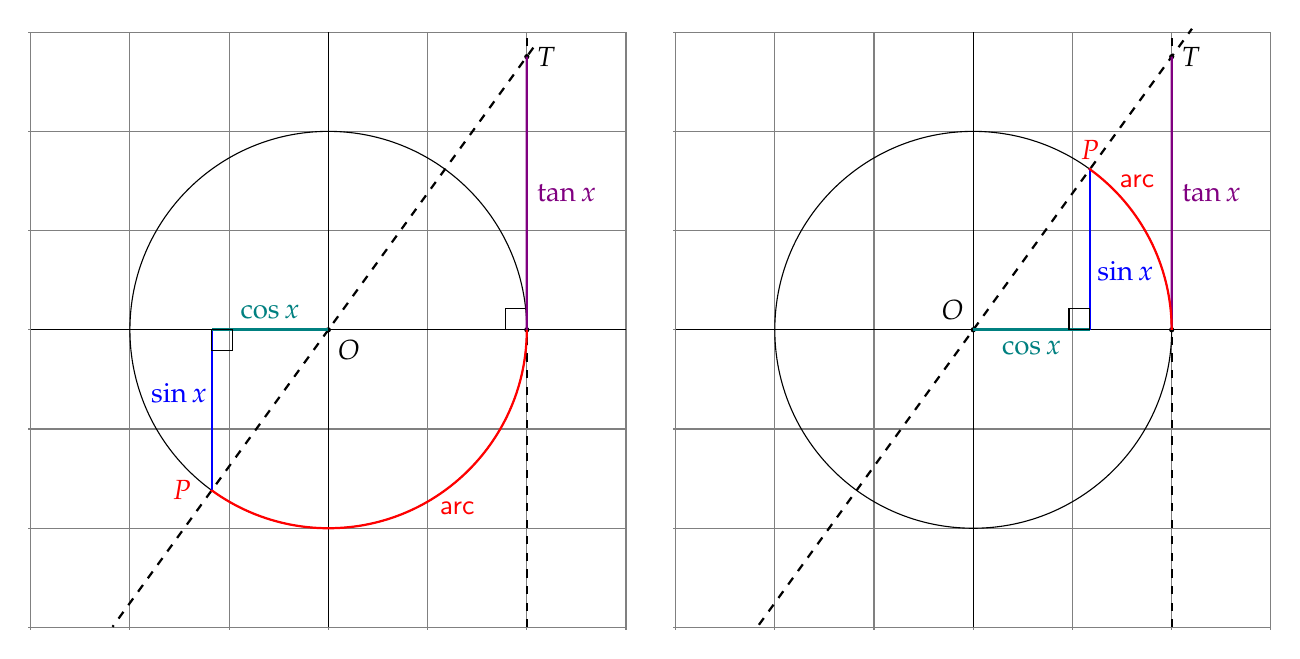
\begin{tikzpicture}[scale=.63]
\begin{scope}
\draw[step=2cm,white!50!black,thin] (-6.05,-6.05) grid (6,6);
\draw[thin] (-6,0) -- (6,0);
\draw[thin] (0,-6) -- (0,6);
  \coordinate (A) at (-4,0);
  \coordinate (B) at (4,0);
  \coordinate[label = below right:$O$] (O) at (0,0);
  \fill (B) circle (1.5pt);
  \fill (O) circle (1.5pt);
  \node[draw, name path = circle] at (O)
    [circle through = (A)] {};
  \coordinate (point) at (-126:7.4);
  \draw[thick,dashed,name path=side] ($(point)!1.95!(O)$) -- (point);
  \draw[dashed,thick,name path=tangent] (4,-6) -- (4,6);
  \path [name intersections = {of = circle and side, by = {dummy,P}}];
  \fill[red] (P) circle (1pt) node[left,xshift=-4pt] {$P$};
  \draw[thick,blue] (P) -- node[left,xshift=2pt,yshift=6pt] {$\sin x$}
    (P |- O) coordinate (Ps);
  \draw[very thick,teal] (O) -- node[above] {$\cos x$} (Ps);
  \draw[rotate=-90] (Ps) rectangle +(12pt,12pt);
  \draw[rotate=90] (B) rectangle +(12pt,12pt);
  \path [name intersections = {of = side and tangent, by = {T}}];
  \fill (T) circle (1.5pt) node[right]     {$T$};
  \draw[thick,violet] (B) -- node[right] {$\tan x$} (T);
  \draw[thick,red] (B) arc[start angle=0, end angle=-126, radius=4cm];
  \node[red] at (2.6,-3.6) {\textsf{arc}};
\end{scope}
\begin{scope}[xshift=13cm]
\draw[step=2cm,white!50!black,thin] (-6.05,-6.05) grid (6,6);
\draw[thin] (-6,0) -- (6,0);
\draw[thin] (0,-6) -- (0,6);
  \coordinate (A) at (-4,0);
  \coordinate (B) at (4,0);
  \coordinate[label = above left:$O$] (O) at (0,0);
  \fill (B) circle (1.5pt);
  \fill (O) circle (1.5pt);
  \node[draw, name path = circle] at (O)
    [circle through = (A)] {};
\coordinate (point) at (54:7.5);
  \draw[thick,dashed,name path=side] ($(O)!-.98!(point)$) -- (point);
  \draw[dashed,thick,name path=tangent] (4,-6) -- (4,6);
  \path [name intersections = {of = circle and side, by = {P}}];
  \fill[red] (P) circle (1pt) node[above] {$P$};
  \draw[thick,blue] (P) -- node[right,xshift=-1pt,yshift=-8pt] {$\sin x$}
    (P |- O) coordinate (Ps);
  \draw[very thick,teal] (O) -- node[below] {$\cos x$} (Ps);
  \draw[rotate=90] (Ps) rectangle +(12pt,12pt);
  \path [name intersections = {of = side and tangent, by = {T}}];
  \fill (T) circle (1.5pt) node[right]     {$T$};
  \draw[thick,violet] (B) -- node[right] {$\tan x$} (T);
  \draw[thick,red] (B) arc[start angle=0, end angle=54, radius=4cm];
  \node[red] at (3.3,3) {\textsf{arc}};
\end{scope}
\end{tikzpicture}
\caption{Signs of the trigonometric functions}\label{fig.signs}
\end{center}
\end{figure}

% !TeX root = trigonometric-functions.tex

\chapter{Translation of the Center and Change of Radius}\label{ch.translated}


Students learning functions also learn about (affine) transformations and their graphical representation.
When they study trigonometric functions, they should be able to plot the graphs $f(x + a)$, $f(ax)$, $f(x)+a$, $af(x)$ for any function $f(x)$.
One can ask: what is the added value of studying the graphical representation of transformations on trigonometric functions?
Here are some reasons:
\begin{itemize}
\item Strengthening their understanding of the trigonometric identities, in particular, their periodic properties.
\item Studying the graphs of the sine and cosine functions as horizontal transformations of each other.
item Identifying the parameters of transformations that can change properties of functions, such as boundedness, period, extrema and zeros.
\end{itemize}

\geoproject{g.transformations} can be used to explore transformations of the unit circle.

%\begin{figure}[hbt]
\begin{wrapfigure}[20]{r}{.5\textwidth}
\begin{center}
\vspace{-4ex}
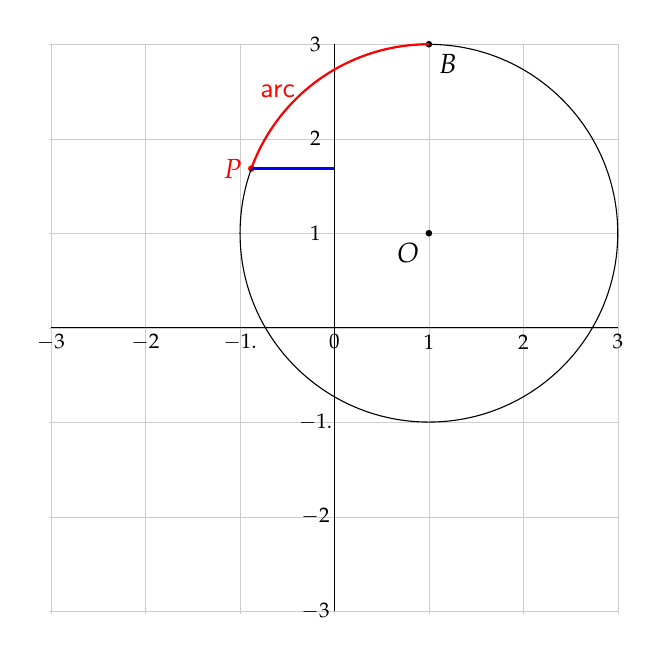
\begin{tikzpicture}[scale=.6]
\draw[step=20mm,white!80!black,ultra thin] (-6.05,-6.05) grid (6,6);
\draw (-6,0) -- (6,0);
\draw (0,-6) -- (0,6);
\foreach \x in {-3,-2,-1.,0,1,2,3}
  \node at (2*\x,-.3) {$\scriptstyle \x$};
\foreach \y in {-3,-2,-1.,1,2,3}
  \node at ($(-.4,0)+(0,2*\y)$) {$\scriptstyle \y$};
\coordinate (O) at (2,2);
\coordinate (B) at (2,6);
\coordinate (P) at ($(2,2)+(160:4)$);
\fill (O) circle(2pt) node [below left] {$O$};
\fill (B) circle(2pt) node [below right] {$B$};
\fill[red] (P) circle(2pt) node [left] {$P$};
\node[draw, name path = circle] at (O)
    [circle through = (P)] {};
\draw[red,thick] (B) arc[start angle=90,end angle=160,radius=4cm];
\node[red] at (-1.2,5) {$\textsf{arc}$};
\coordinate (origin) (0,0);
\draw[blue,thick] (P) -- (P -| origin);
\end{tikzpicture}
%\includegraphics[width=\textwidth,keepaspectratio]{translation-of-the-unit-circle}
\caption{Transformations of the unit circle: center $(1,1)$, radius $3$, initial point $(3,1)$}\label{fig.transformations-of-the-unit-circle}
\end{center}
%\end{figure}
\end{wrapfigure}

The project displays two windows. The left window  (Figure~\ref{fig.transformations-of-the-unit-circle}) includes sliders (not shown in the Figure) that enable the user to translate the center of the circle $O$ (here to $(1,1)$), expand or contract the radius (here $2$) and to choose a point $B$ to start the winding (here $(1,3)$).

The right window (Figure~\ref{fig.trace-of-a-transformation-of-the-unit-circle}) shows a trace of the value of a function, as the point $X$ is moved along the $x$-axis. You can select either $F_x$ to show the $x$ value of $P$ or $F_y$ to show the $y$ value of $P$.

\begin{figure}[hbt]
\begin{center}
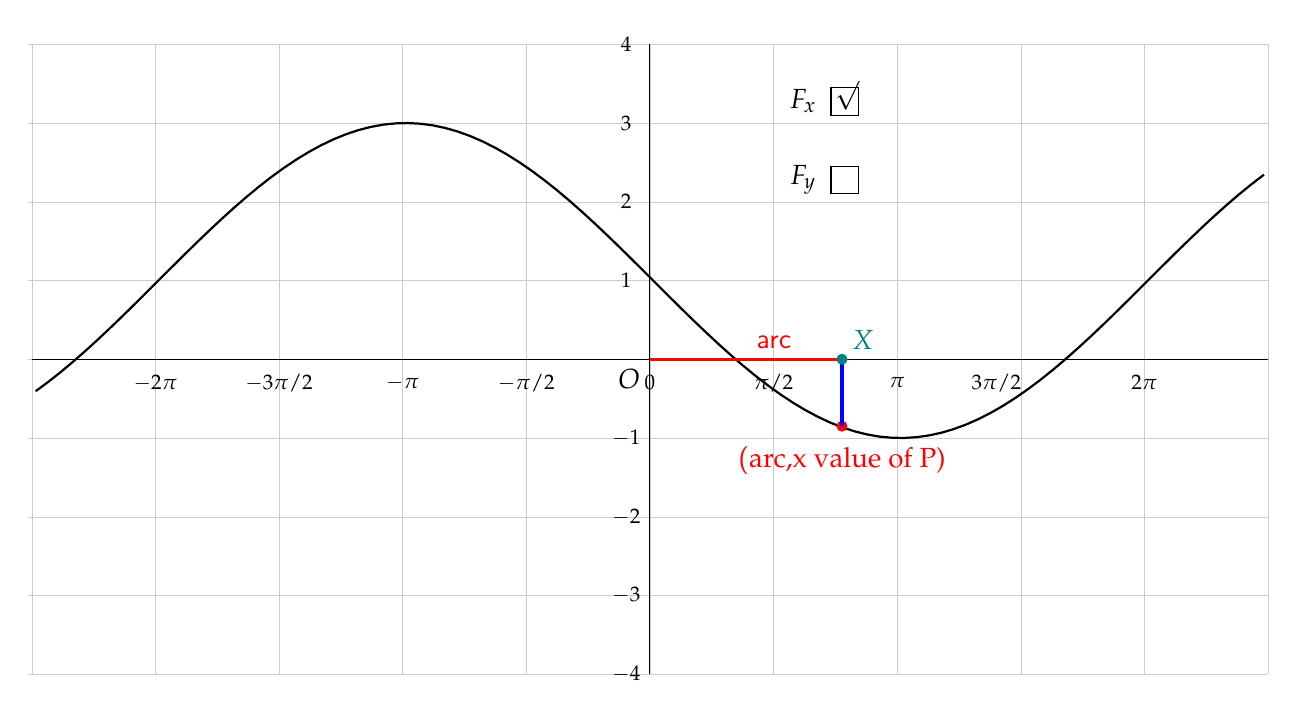
\begin{tikzpicture}
\draw[xstep=1.57cm,ystep=1cm,white!80!black,ultra thin] (-7.9,-4) grid (7.85,4);
\draw (-7.85,0) -- (7.85,0);
\draw (0,-4) -- (0,4);
\foreach \x/\tick in {-6.28/{-2\pi},-4.71/{-3\pi/2},-3.14/{-\pi},-1.57/{-\pi/2},0/0,1.57/{\pi/2},3.14/{\pi},4.4/{3\pi/2},6.28/{2\pi}}
  \node at (\x,-.3) {$\scriptstyle\tick$};
\foreach \y in {-4,-3,-2,-1,1,2,3,4}
  \node at ($(-.3,0)+(0,\y)$) {$\scriptstyle\y$};
\draw[thick,domain=-7.8:7.8,samples=100] plot (\x,{2*cos (.5*(\x+3.1) r)+1});
\coordinate (P) at (2.44,-.85);
\coordinate (O) at (0,0);
\node [below left] at (O) {$O$};
\fill[red] (P) circle(2pt) node [below,yshift=-4pt] {\textsf(arc,x value of P)};
\draw [very thick,blue] (P) -- (P |- O) coordinate (X);
\draw[very thick,red] (O) -- node[above right] {\textsf{arc}} (X);
\fill[teal] (X) circle(2pt) node[above right] {$X$};

\draw (2.3,3.1) rectangle +(10pt,10pt) node[xshift=-20pt,yshift=-5pt] {$F_x$}
  node[xshift=-4pt,yshift=-3pt] {$\surd$};
\draw (2.3,2.1) rectangle +(10pt,10pt) node[xshift=-20pt,yshift=-5pt] {$F_y$};
\end{tikzpicture}
%\includegraphics[width=\textwidth,keepaspectratio]{trace-of-translation-of-the-unit-circle}
\caption{Trace of a transformation of the unit circle}\label{fig.trace-of-a-transformation-of-the-unit-circle}
\end{center}
\end{figure}

We recommend beginning the exploration with the unit circle centered at the origin with starting point $B$ at $(1,0)$ and then changing one parameter at a time.
For example, changing either the $x$ or $y$ value of the center of the circle (but not both) and asking students to predict the change in the graph of the function.
Next, return the center to the origin, changing the starting point $B$.

Assuming that the students have experience in transformations of functions, you can ask them to predict the algebraic expression corresponding to the transformed function.
For example, if we only change the $x$ value of the center of the circle to $1$,  the function $F_y$ remains $\sin x$, since the $y$ value of a point $P$ depends only on the length of the arc from $B$ and not on the center.
Similarly, if $B$ is moved to $(0,1)$ the function $F_x$ becomes $\cos\left(x + \disfrac{\pi}{2}\right)$.\footnote{To erase the trace and start over, move the right window with the mouse. To reset the parameters of the circle, click on the curved arrow symbol at the top right of the left window.}

Changing the radius should be the last transformation explored, because it changes both the amplitude and the cycle of the resulting function.
For changes shown in Figure~\ref{fig.transformations-of-the-unit-circle}, the function in Figure~\ref{fig.trace-of-a-transformation-of-the-unit-circle} is:
\[
3\cos\left(\frac{(x-1)+\pi/2}{3}\right)+1\,.
\]

An interesting research question is to ask if it possible to get all possible translations, expansions and contractions of the trigonometric functions only by changing these parameters.



% !TeX root = trigonometric-functions.tex

\chapter{Analysis of Trigonometric Functions}\label{ch.analysis}

There are two approaches to obtaining the derivative of the trigonometric functions: geometric and algebraic. We will use both approaches to prove that $\sin' x=\cos x$:
\[
\lim_{x \rightarrow 0} \disfrac{\sin (x+h)-\sin x}{h}\stackrel{?}{=}\cos x\,.
\]
In both cases, we need a fundamental concept: as the length of an arc tends to zero, the ratio of the arc to the chord with the same endpoints tends to one.

\section{The ratio of the length of an arc to its chord}

Figure~\ref{fig.arcs-and-chords} shows four arcs and the chords with the same endpoints. The arcs subtend central angles of $80^\circ, 60^\circ, 40^\circ, 5^\circ$. As the arcs get smaller, the difference between the length of the arc and the length of the chord is harder to see. Of course this is what we want, but it is difficult to give an estimate of this difference.

\begin{figure}[hbt]
\begin{center}
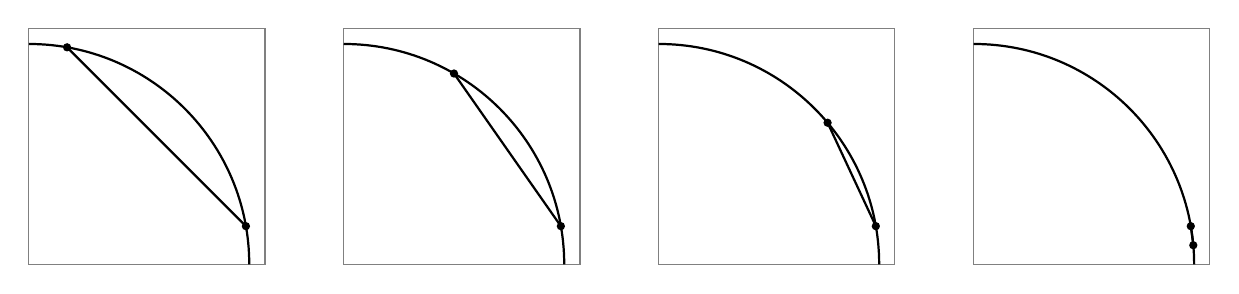
\begin{tikzpicture}
\draw[thin,white!50!black] (0,0) rectangle +(3,3);
\draw[thick] (2.8,0) arc[start angle=0,end angle=90,radius=2.8cm];
\coordinate (s1) at (10:2.8);
\fill (s1) circle (1.5pt);
\coordinate (t1) at (80:2.8);
\fill (t1) circle (1.5pt);
\draw[thick] (s1) -- (t1);
\begin{scope}[xshift=4cm]
\draw[thin,white!50!black] (0,0) rectangle +(3,3);
\draw[thick] (2.8,0) arc[start angle=0,end angle=90,radius=2.8cm];
\coordinate (s2) at (10:2.8);
\fill (s2) circle (1.5pt);
\coordinate (t2) at (60:2.8);
\fill (t2) circle (1.5pt);
\draw[thick] (s2) -- (t2);
\end{scope}
\begin{scope}[xshift=8cm]
\draw[thin,white!50!black] (0,0) rectangle +(3,3);
\draw[thick] (2.8,0) arc[start angle=0,end angle=90,radius=2.8cm];
\coordinate (s3) at (10:2.8);
\fill (s3) circle (1.5pt);
\coordinate (t3) at (40:2.8);
\fill (t3) circle (1.5pt);
\draw[thick] (s3) -- (t3);
\end{scope}
\begin{scope}[xshift=12cm]
\draw[thin,white!50!black] (0,0) rectangle +(3,3);
\draw[thick] (2.8,0) arc[start angle=0,end angle=90,radius=2.8cm];
\coordinate (s4) at (5:2.8);
\fill (s4) circle (1.5pt);
\coordinate (t4) at (10:2.8);
\fill (t4) circle (1.5pt);
\draw[thick] (s4) -- (t4);
\end{scope}
\end{tikzpicture}
\caption{Arcs and the corresponding chords}\label{fig.arcs-and-chords}
\end{center}
\end{figure}
It might be easier to envision the convergence of arcs and chords by examining  regular polygons inscribed within a circle (Figure~\ref{fig.regular-polygons}, \geoproject{g.polygon}).

\begin{figure}[hbt]
\begin{center}
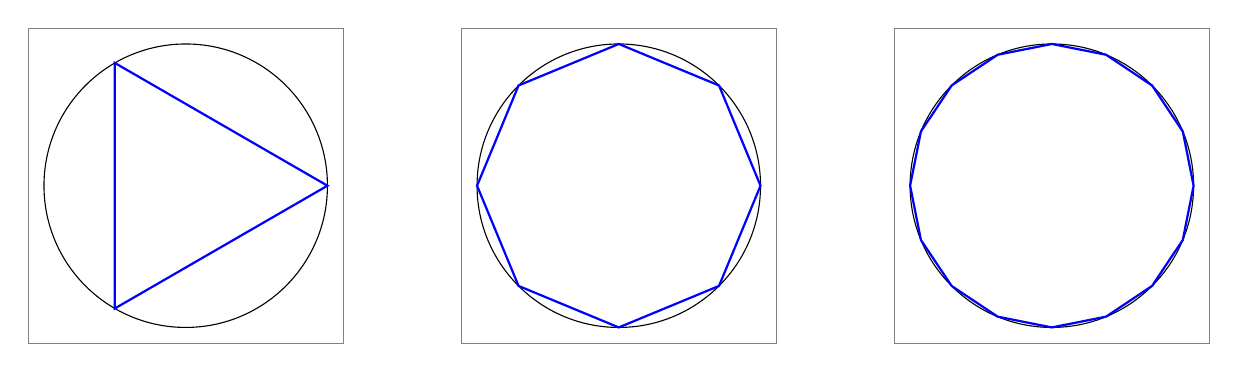
\begin{tikzpicture}
\draw[thin,white!50!black] (-2,-2) rectangle +(4,4);
\coordinate (o1) at (0,0);
\coordinate (a1) at (1.8,0);
\node[draw, name path = circle] at (o1)
    [circle through = (a1)] {};
\foreach \node/\angle in {a2/120,a3/240} {
  \coordinate (\node) at (\angle:1.8);
}
\draw[thick,blue] (a1) -- (a2) -- (a3) -- cycle;
\begin{scope}[xshift=5.5cm]
\draw[thin,white!50!black] (-2,-2) rectangle +(4,4);
\coordinate (o2) at (0,0);
\coordinate (b1) at (1.8,0);
\node[draw, name path = circle] at (o2)
    [circle through = (b1)] {};
\foreach \node/\angle in
  {b2/45,b3/90,b4/135,b5/180,b6/-135,b7/-90,b8/-45} {
  \coordinate (\node) at (\angle:1.8);
}
\draw[thick,blue] (b1) -- (b2) -- (b3) -- (b4) -- (b5) -- (b6) -- (b7) -- (b8) -- cycle;
\end{scope}
\begin{scope}[xshift=11cm]
\draw[thin,white!50!black] (-2,-2) rectangle +(4,4);
\coordinate (o3) at (0,0);
\coordinate (c1) at (1.8,0);
\node[draw, name path = circle] at (o3)
    [circle through = (c1)] {};
\foreach \node/\angle in
  {c2/22.5,c3/45,c4/67.5,c5/90,c6/112.5,c7/135,
   c8/157.5,c9/180,c16/-22.5,c15/-45,c14/-67.5,
   c13/-90,c12/-112.5,c11/-135,c10/-157.5} {
  \coordinate (\node) at (\angle:1.8);
}
\draw[thick,blue] (c1) -- (c2) -- (c3) -- (c4) -- (c5) -- (c6) --
  (c7) -- (c8) -- (c9) -- (c10) -- (c11) -- (c12) -- (c13) --
  (c14) -- (c15) -- (c16) -- cycle;
\end{scope}
\end{tikzpicture}
%\includegraphics[width=\textwidth,keepaspectratio]{figure21}
\caption{Regular polygons inscribed within a circle}\label{fig.regular-polygons}
\end{center}
\end{figure}

The more sides in the polygon, the closer its perimeter is to the circumference of the circle.
The circumference of the circle divided by the number of sides is the length of an arc with the same endpoints as the corresponding side.
(In a regular polygon, all sides have the same length.)
Since the ratio of the circumference of the circle to the perimeter of an inscribed polygon approaches 1 as the number of sides increases, so does the ratio of the length of an arc to the corresponding chord.

To check this numerically, let us compute the length of an arc, the length of the corresponding chord and their ratio.
The length of an arc subtending an angle of $x$ degrees is $2\pi\disfrac{x}{360}$.

%\begin{figure}[H]
\begin{wrapfigure}{r}{.5\textwidth}
\begin{center}
\vspace{-3ex}
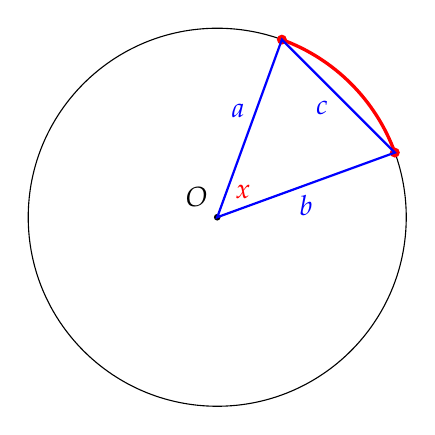
\begin{tikzpicture}[scale=1.2]
  \coordinate  (A) at (-2,0);
  \coordinate[label = above left:$O$] (O) at (0,0);
  \fill (O) circle (1pt) node[above right,red,xshift=3pt,yshift=3pt] {$x$};
  \node[draw, name path = circle] at (O)
    [circle through = (A)] {};
  \coordinate (P) at (20:2);
  \fill[red] (P) circle (1.5pt);
  \coordinate (Q) at (70:2);
  \fill[red] (Q) circle (1.5pt);
  \draw[red,very thick] (P)
    arc[start angle=20,end angle=70,radius=2cm];
  \draw[thick,blue] (P) -- node[below left,yshift=2pt] {$c$} (Q) -- 
    node[above left,xshift=2pt] {$a$} (O) -- node[below] {$b$} cycle;
\end{tikzpicture}
\caption{The length of a chord corresponding to an arc of size $x$}\label{fig.length-of-a-chord}
\end{center}
%\end{figure}
\end{wrapfigure}
By the law of cosines the length of a chord $c$ subtending is (Figure~\ref{fig.length-of-a-chord}):
\[
c^2=a^2+b^2-2ab\cos x\,.
\]

In the unit circle $a=b=1$ so:
\[
c=\sqrt{2-2\cos x}\,.
\]
For the arcs and chords in Figure~\ref{fig.arcs-and-chords}:
\[
\begin{array}{|r|r|r|r|}
\hline
\multicolumn{1}{|c}{\textrm{Angle}} &
\multicolumn{1}{|c}{\textrm{Arc length}} &
\multicolumn{1}{|c}{\textrm{Chord length}} &
\multicolumn{1}{|c|}{\textrm{Ratio}}\\\hline
80 & 1.396 & 1.286  & 1.090\\\hline
60 & 1.047 & 1.000  & 1.047\\\hline
40 & 0.698 & 0.684 & 1.006\\\hline
5  & 0.087 & 0.087 &1.000 \\\hline
\end{array}
\]

%\begin{figure}[H]
\begin{wrapfigure}[12]{r}{.5\textwidth}
\begin{center}
\vspace{-3ex}
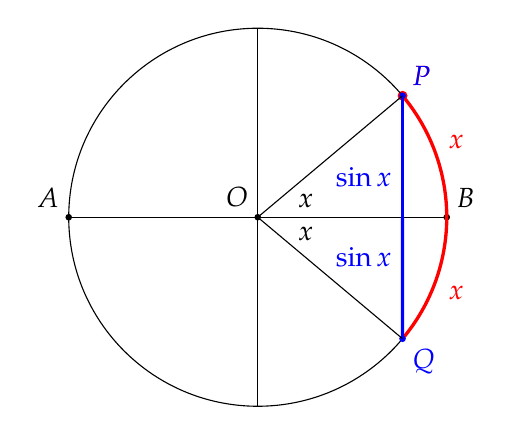
\begin{tikzpicture}[scale=1.2]
  \draw[thin] (-2,0) -- (2,0);
  \draw[thin] (0,-2) -- (0,2);
  \coordinate[label = above left:$A$]  (A) at (-2,0);
  \coordinate[label = above right:$B$] (B) at (2,0);
  \coordinate[label = above left:$O$] (O) at (0,0);
  \fill (A) circle (1pt);
  \fill (B) circle (1pt);
  \fill (O) circle (1pt) node[above right,xshift=11pt] {$x$} 
    node[below right,xshift=11pt] {$x$};
  \coordinate (P) at (40:2);
  \fill[red] (P) circle (1.5pt) node[above right] {$P$};
  \coordinate (Q) at (-40:2);
  \node[draw, name path = circle] at (O)
    [circle through = (A)] {};
  \draw[red,very thick] (B)
    arc[start angle=0,end angle=40,radius=2cm];
  \draw[red,very thick] (B)
    arc[start angle=0,end angle=-40,radius=2cm];
  \node[red] at (2.1,.8) {$x$};
  \node[red] at (2.1,-.8) {$x$};
  \draw[very thick,blue] (P) -- node[below left] {$\sin x$}
    (P |- O) coordinate (D);
  \draw[very thick,blue] (D) -- node[above left] {$\sin x$} (Q);
%  \fill (D) circle (1pt) node[below right] {$D$};
  \fill[blue] (P) circle (1pt) node[above right] {$P$};
  \fill[blue] (Q) circle (1pt) node[below right] {$Q$};
  \draw (Q) -- (O) -- (P);
\end{tikzpicture}
%\includegraphics[width=.5\textwidth,keepaspectratio]{figure22}
\caption{Ratio of $\sin x$ to $x$}\label{fig.ratio-of-sine-to-x}
\end{center}
%\end{figure}
\end{wrapfigure}

\bigskip

Let us now compute:
\[
\lim_{x \rightarrow 0} \disfrac{\sin x}{x} = \lim_{x \rightarrow 0} \disfrac{2\sin x}{2x}\,.
\]
From Figure~\ref{fig.ratio-of-sine-to-x} we see that this is the ratio the length of the chord $PQ$ to the length of the arc $PQ$.
But we have shown that this ratio converges to $1$ as the subtended angle $2x$ tends to $0$. Therefore:
\[
\lim_{x \rightarrow 0} \disfrac{\sin x}{x} = 1\,.
\]

\bigskip\bigskip\bigskip

\section{The geometric approach}
The limit
\[
\lim_{x \rightarrow 0} \disfrac{\sin (x+h)-\sin x}{h}
\]
is computed by looking at the geometric meaning of each component of the expression.
In Figure~\ref{fig.geometric-computation}, $x$ is the length of the arc from $B$ to $P_x$, $h$ is the length of the arc from $P_x$ to $P_{x+h}$; by adding the arc lengths, $x+h$ is the length of the arc from $B$ to $P_{x+h}$.
Note that the length of an arc in the unit circle is the same as the central angle (in radians) that it subtends.

\begin{figure}[hbt]
\begin{center}
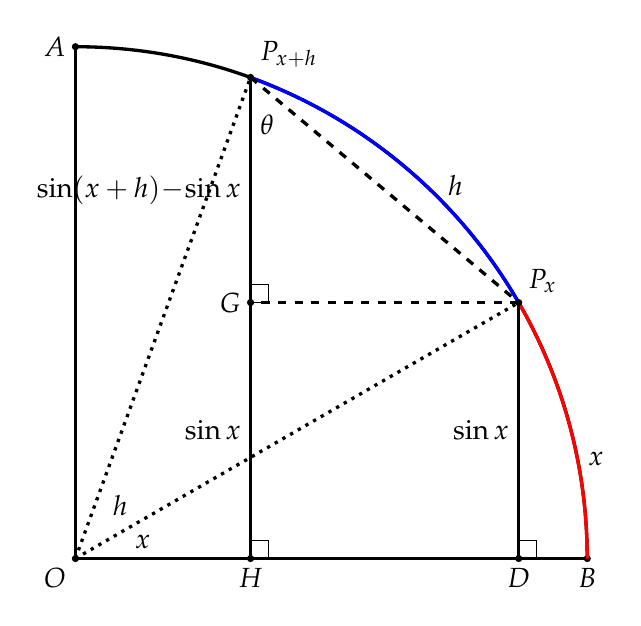
\begin{tikzpicture}[scale=.65]
\coordinate (O) at (0,0);
\coordinate (A) at (0,10);
\coordinate (B) at (10,0);
\fill (O) circle (2pt)
  node[below left] {$O$}
  node[right,xshift=18pt,yshift=6pt] {$x$}
  node[above right,xshift=10pt,yshift=12pt] {$h$};
\fill (A) circle (2pt) node[left] {$A$};
\fill (B) circle (2pt) node[below] {$B$};

\draw[very thick,name path=axes] (B) -- (O) -- (A);
\draw[very thick,name path=arc] (10,0)
  arc[start angle=0, end angle=90, radius=10]
  node[very near start,right] {$x$}
  node[midway,right,yshift=4pt] {$h$};
\draw[very thick,red] (10,0)
  arc[start angle=0, end angle=30, radius=10];
\draw[very thick,blue] (30:10)
  arc[start angle=30, end angle=70, radius=10];

\path[name path=px] (O) -- (30:11);
\path [name intersections={of=arc and px,by={Px}}];
\fill (Px) circle (2pt) node[above right] {$P_x$};

\draw[very thick,name path=pxd] (Px) -- (Px |- O);
\path[name intersections={of=pxd and axes,by={D}}];
\fill (D) circle (2pt) node[below] {$D$};

\path[name path=pxh] (O) -- (70:11);
\path [name intersections={of=arc and pxh,by={Pxh}}];
\fill (Pxh) circle (2pt)
  node[above right] {$P_{x+h}$}
  node[below right,yshift=-10pt] {$\theta$};

\draw[very thick,name path=pxh] (Pxh) -- (Pxh |- O);
\path [name intersections={of=pxh and axes,by={H}}];
\fill (H) circle (2pt) node[below] {$H$};

\draw[very thick,dashed,name path=pxpxh] (Px) -| (Pxh);
\path [name intersections={of=pxh and pxpxh,by={G}}];
\fill (G) circle (2pt) node[left] {$G$};

\draw (D) rectangle +(10pt,10pt);
\draw (G) rectangle +(10pt,10pt);
\draw (H) rectangle +(10pt,10pt);

\draw[very thick,dotted] (O) -- (Pxh);
\draw[very thick,dotted] (O) -- (Px);
\draw[very thick,dashed] (Pxh) -- (Px);

\path (D) -- node[left] {$\sin x$} (Px);
\path (H) -- node[left] {$\sin x$} (G);
\path (G) -- node[left] {$\sin(x+h)\!-\!\sin x$} (Pxh);
\end{tikzpicture}
\caption{Geometric computation of the limit}\label{fig.geometric-computation}
\end{center}
\end{figure}

$P_xD$ and $P_{x+h}H$ are perpendicular to the $x$-axis and $P_xG$ is perpendicular to $P_{x+h}H$.
We are interested in the angle $\theta$, which is the difference between two angles:
\[
\theta=\angle GP_{x+h}P_x= \angle OP_{x+h}P_x - \angle OP_{x+h}H\,.
\]
All radii are equal so $\triangle OP_{x+h}P_x$ is isoceles, and the sum of the angles of a triangle is $\pi$:
\[
\angle OP_{x+h}P_x=\frac{1}{2}(\pi - h)\,.
\]
From the sum of the angles in the right triangle $\triangle OP_{x+h}H$ we have:
\[
\angle OP_{x+h}H = \left(\pi-\frac{\pi}{2}-(x+h)\right) = \left(\frac{\pi}{2}-(x+h)\right)\,.
\]
Therefore:
\[
\theta = \frac{1}{2}(\pi - h) - \left(\frac{\pi}{2}-(x+h)\right) = x+\frac{h}{2}\,.
\]

\smallskip

In the right triangle $\triangle P_xGP_{x+h}$:
\[
\cos \theta = \frac{P_{x+h}G}{P_{x+h}P_x}=\frac{\sin(x+h)\!-\!\sin x}{P_{x+h}P_x}\approx \frac{\sin(x+h)\!-\!\sin x}{h}\,,
\]
taking the length of the arc $h$ as an approximation of the chord $P_xP_{x+h}$. Taking the limit:
\[
\sin' x = \lim_{h\rightarrow 0} \frac{\sin(x+h)\!-\!\sin x}{h} =  \lim_{h\rightarrow 0}\cos \theta = \lim_{h\rightarrow 0} \cos \left(x+\frac{h}{2}\right) = \cos x\,.
\]

\section{The algebraic approach}

We use the identity:
\[
\sin(\alpha) -\sin\beta = 2\sin \frac{\alpha-\beta}{2}\cos \frac{\alpha+\beta}{2}\,,
\]
and the continuity of both the sine and cosine functions:
\begin{eqnarray*}
\lim_{h\rightarrow 0} \frac{\sin(x+h)\!-\!\sin x}{h}&=& \lim_{h\rightarrow 0} \frac{2\sin(\frac{h}{2})\cos(\frac{2x+h}{2})}{h}\\
&=&\lim_{h\rightarrow 0}
  \left[
    \left( 
      \frac{\sin(\frac{h}{2})}{\frac{h}{2}}
    \right)
    \cos\left( x+\frac{h}{2} \right)
   \right]\\
& =& \cos x\,.
\end{eqnarray*}
Students can be asked to justify each of the steps in this computation.

\bigskip

The choice between the two approaches depends on the which skills we wish to reinforce in the students.
Clearly, the geometric approach requires the ability to follow a non-trivial geometric derivation. 
The algebraic approach depends on understanding the concepts of continuity and limits.

We emphasize that both approaches are based on:
\[
\lim_{h\rightarrow 0} \frac{\sin(x+h)\!-\!\sin x}{h} =1
\]
that was proved at the beginning of this chapter.

\bigskip

We refer the reader to the article by Josevich \cite{josevich} who shows how the derivative can be obtained from the principles of classical mechanics.

% !TeX root = trigonometric-functions.tex

\chapter{Additional Topics}



\section{The secant and cosecant functions}

The functions secant and cosecant are usually defined on right triangles as the inverses $\sec x = \disfrac{1}{\cos x}$, $\csc x = \disfrac{1}{\sin x}$.
Can these functions can be defined geometrically?
In other words, from the construction of the trigonometric functions (Figure~\ref{fig.secant-and-cosecant}), can we find their lengths?
We claim that $OT=|\sec x|$ and $OC=|\csc x|$. 

\begin{figure}[H]
\begin{center}
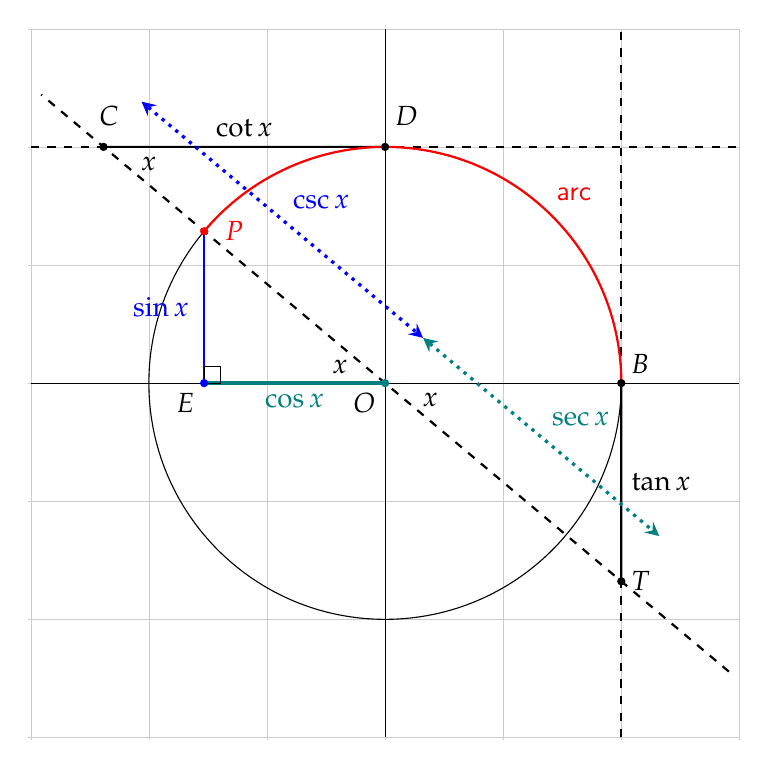
\begin{tikzpicture}[scale=.75]
\draw[step=2cm,white!80!black,ultra thin] (-6.05,-6.05) grid (6,6);
\draw[thin] (-6,0) -- (6,0);
\draw[thin] (0,-6) -- (0,6);
  \coordinate (A) at (-4,0);
  \coordinate (B) at (4,0);
  \coordinate (D) at (0,4);
  \coordinate (O) at (0,0);
  \node[draw, name path = circle] at (O)
    [circle through = (A)] {};
  \coordinate (point) at (140:7.6);
  \draw[thick,dashed,name path=side] ($(point)!2!(O)$) -- (point);
  \draw[dashed,thick,name path=tangent] (4,-6) -- (4,6);
  \draw[dashed,thick,name path=cotangent] (-6,4) -- (6,4);
  \path [name intersections = {of = circle and side, by = {P}}];
  \draw[thick,blue] (P) -- (P |- O) coordinate (Ps);
  \path[blue] (P) --  node[left,xshift=-2pt] {$\sin x$}  (Ps);
  \draw[very thick,teal] (O) -- node[below] {$\cos x$} (Ps);
  \draw (Ps) rectangle +(8pt,8pt);
  \path [name intersections = {of = side and tangent, by = {T}}];
  \draw[thick] (B) -- node[right] {$\tan x$} (T);
  \path [name intersections = {of = side and cotangent, by = {C}}];
  \draw[thick] (D) -- node[above] {$\cot x$} (C);
  \draw[thick,red] (B)
    arc[start angle=0, end angle=140, radius=4cm];
  \node[red] at (3.2,3.2) {\textsf{arc}};

  \coordinate (C1) at ($(C)+(230:-1)$);
  \coordinate (O1) at ($(O)+(230:-1)$);
  \coordinate (T1) at ($(T)+(230:-1)$);
  \draw[very thick,blue,dotted,<->] (C1) -- 
    node[above right] {$\csc x$} (O1);
  \draw[very thick,teal,dotted,<->] (O1) -- 
    node[above right] {$\sec x$} (T1);

  \fill (B) circle (2pt) node[above right] {$B$};
  \fill[blue] (Ps) circle (2pt) node[below left,black] {$E$};
  \fill[teal] (O) circle (2pt) node[below left,black] {$O$}
        node[above left,xshift=-10pt,black] {$x$}
        node[below right,xshift=10pt,black] {$x$};;
  \fill (D) circle (2pt) node[above right,yshift=4pt] {$D$};
  \fill (T) circle (2pt) node[right]     {$T$};
  \fill (C) circle (2pt) node[above,xshift=2pt,yshift=4pt] {$C$}
    node[below right,xshift=10pt] {$x$};
  \fill[red] (P) circle (2pt) node[right,xshift=4pt] {$P$};
\end{tikzpicture}
\caption{The secant and cosecant functions}\label{fig.secant-and-cosecant}
\end{center}
\end{figure}

Here is the proof that $OC=\csc x$:
\begin{itemize}
\item Radii of the unit circle: $OP = OD =1$.
\item By construction: $PE = \sin x$.
\item $CD \parallel EO$ so the alternate interior angles $\angle DCO, \angle EOC$ are equal.
\item Therefore, $\triangle PEO \sim \triangle ODC$, so:
\[
\frac{OC}{OP} = \frac{OD}{PE}=\left|\frac{1}{\sin x}\right|\,,\;\;\;\;\;
OC = 1\cdot\left|\disfrac{1}{\sin x}\right|=|\csc x|\,.
\]
\end{itemize}
A similar proof shows that $\triangle PEO \sim \triangle TBO$, so $OT = \left|\disfrac{1}{\cos x}\right|=|\sec x|$.



\section{From functions to triangles}

Even when beginning the study of trigonometry with the functional approach, at some point the transition to the functions on right triangles must be done.
This is very easy since the the measure of an arc is the same as the measure (in radians) of the central angle it subtends.

\begin{wrapfigure}[14]{r}{.5\textwidth}
\begin{center}
\vspace{-4ex}
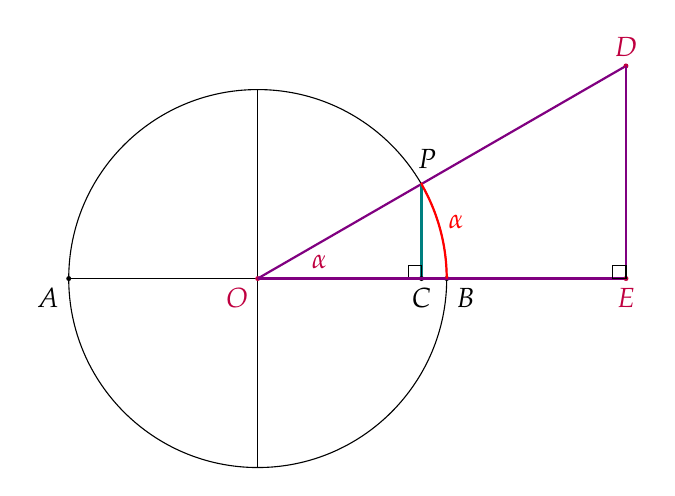
\begin{tikzpicture}[scale=.6]
\draw[thin] (-4,0) -- (7.8,0);
\draw[thin] (0,-4) -- (0,4);
  \coordinate[label=below left:$A$] (A) at (-4,0);
  \coordinate[label=below right:$B$] (B) at (4,0);
  \coordinate (O) at (0,0);
  \fill (A) circle (1.5pt);
  \fill (B) circle (1.5pt);
  \fill[purple] (O) circle (1.5pt) 
    node[below left] {$O$}
    node[above right,xshift=16pt] {$\alpha$};
  \node[draw, name path = circle] at (O)
    [circle through = (A)] {};
  \coordinate (D) at (30:9);
  \draw[thick,violet,name path=side] (O) -- (D);
  \fill[purple] (D) circle (1.5pt) node[above] {$D$};;
  \path [name intersections = {of = circle and side, by = {P}}];
  \fill[red] (P) circle (1pt) node[black,above,xshift=2pt,yshift=2pt] {$P$};
  \draw[thick,teal] (P) -- (P |- O) coordinate (C);
  \fill (C) circle (1.5pt) node[below] {$C$}; 
  \draw[rotate=90] (C) rectangle +(8pt,8pt);
  \draw[thick,violet] (D) -- (D |-  O) coordinate (E) -- (O);
  \fill[purple] (E) circle (1.5pt) node[below] {$E$}; 
  \draw[rotate=90] (E) rectangle +(8pt,8pt);
  \draw[thick,red] (B) arc[start angle=0, end angle=30, radius=4cm];
  \node[red] at (4.2,1.2) {$\alpha$};
\end{tikzpicture}
\caption{From functions to right triangles}\label{fig.functions-to-triangles}
\end{center}
\end{wrapfigure}
Any right triangle can be embedded in a coordinate system such that one side rests of the $x$-axis with the adjacent acute angle at the origin, as shown by $\triangle DEO$ in Figure~\ref{fig.functions-to-triangles}.
(Recall that in a right triangle two angles are acute.)
Now construct a unit circle centered at the origin and drop a perpendicular from point $P$, the intersection of the circle and the hypotenuse $OD$, to side $OE$.

Since $\angle DEO=\angle PCO=\pi$ and $\angle DOE=\angle POC=\alpha$,  $\triangle DEO\sim \triangle PCO$, so:
\[
\frac{PC}{OP}=\frac{DE}{OD}\,.
\]
$OP = 1$, the radius of the unit circle and$PC = \sin \alpha$ by definition, so $\rule[-10pt]{0pt}{28pt}\disfrac{DE}{OD}=\sin\alpha$.
Therefore, the sine of $\alpha$ \emph{in the triangle} $\triangle DEO$ is equal to the opposite side divided by the hypotenuse, as expected.

Similar arguments show that $\disfrac{OE}{OD}=\cos\alpha$ and $\disfrac{DE}{OE}=\tan \alpha$.

\appendix
% !TeX root = trigonometric-functions.tex

\appendix
\chapter{Geogebra Projects}\label{a.geogebra}

\begin{center}
\begin{tabular}{|r|p{7cm}|p{6cm}|}
\hline
Project & Title & Link\\
\hline
\ref{g.covariance} & Covariance in a right triangle & 
  \url{https:}\\\hline

\ref{g.definition-of-trig-functions} & Definition of the trigonometric functions & 
  \url{https:}\\\hline

\ref{g.winding} & Winding a thread around a polygon &
  \url{https:}\\\hline

\ref{g.sine} & Sine function & 
  \url{https:}\\\hline

\ref{g.single} & Single-screen project & 
  \url{https:}\\\hline

\ref{g.split} & Split-screen project & 
  \url{https:}\\\hline

\ref{g.trace} & Trace of the function & 
  \url{https:}\\\hline

\ref{g.cosine} & Cosine function & 
  \url{https:}\\\hline

\ref{g.tangent} & Tangent function & 
  \url{https:}\\\hline

\ref{g.cotangent} & Cotangent function &
  \url{https:}\\\hline

\ref{g.signs} & Signs of the trignometric functions &
  \url{https:}\\\hline

\ref{g.transformations} & Transformations of the unit circle &
  \url{https:}\\\hline

\ref{g.polygon} & Regular polygons inscribed within a circle & 
  \url{https:}\\\hline
\end{tabular}
\end{center}

% !TeX root = trigonometric-functions.tex

\chapter{``Simple'' Proofs}\label{a.simple}

Chapter~\ref{ch.analysis} presents a relatively complicated geometric proof that $\sin' x=\cos x$ with a relatively simple algebraic proof. However, the comparison is misleading, because the algebraic proof uses the formula for $\sin(x+h)$ which has a relatively complicated geometric proof. The formula for $\sin(x+h)$ is extremely useful as a ``lemma,'' here enabling the simple algebraic proof. This demonstrates the cumulative nature of mathematics, where proofs depend upon the corpus of existing theorems.

Here we present an adaptation of the proof of the formula for $\sin(x+h)$ that is based on Figure~\ref{fig.geometric-computation} used in the geometric proof of $\sin' x=\cos x$. This shows that the proof of this formula is of similar complexity to that of the geometric proof that $\sin' x=\cos x$.

Figure~\ref{fig.simple} is the same as Figure~\ref{fig.geometric-computation} in the sense that no points or lines have been removed or renamed. We have added three line segments. Thick lines are used for the new segments, as well as for several of the existing ones.

Add the following three lines and points ($X,Y,Z$) to the construction:
\begin{itemize}
\item A perpendicular $P_{x+h}X$ from $P_{x+h}$ to $OP_x$. The blue right triangle $\triangle P_{x+h}XO$ is created.
\item A perpendicular $XY$ from $X$ to $P_{x+h}H$. The red right triangle $\triangle P_{x+h}YX$ is created.
\item A perpendicular $XZ$ from $X$ to $OB$. The olive right triangle $\triangle XZO$ is created.
\end{itemize}
The blue triangle is slightly offset so that the reader can see all three triangles.

$\angle YXO=\angle XOB=x$ by alternate interior angles and $\angle YP_{x+h}X=\angle YXO=x$ by a simple computation. The construction is within the unit circle so $OP_{x+h}=1$.

In the blue triangle $\triangle P_{x+h}XO$, $XP_{x+h}=\sin h, OX=\cos h$.

In the red triangle $\triangle P_{x+h}YX$:
\begin{eqnarray*}
\cos x  &=& \frac{YP_{x+h}}{XP_{x+h}}
              = \frac{YP_{x+h}}{\sin h}\\
YP_{x+h}&=& \cos x\sin h\,.
\end{eqnarray*}
In the olive triangle $\triangle XZO$:
\begin{eqnarray*}
\sin x &=& \frac{ZX}{OX}
             = \frac{ZX}{\cos h}\\
ZX     &=& \sin x\cos h\,.
\end{eqnarray*}
$XYHZ$ is a rectangle so $HY=ZX=\sin x \cos y$. Then:
\begin{eqnarray*}
\sin(x+h) &=& \frac{HP_{x+h}}{OP_{x+h}}
                = \frac{HP_{x+h}}{1}
                = HY+YP_{x+h}\\
          &=& \sin x \cos h+\cos x\sin h\,.
\end{eqnarray*}

\newpage
\begin{center}
\textbf{\large Print the Figure in color!}
\end{center}

\bigskip
\bigskip

\begin{figure}[H]
\begin{center}
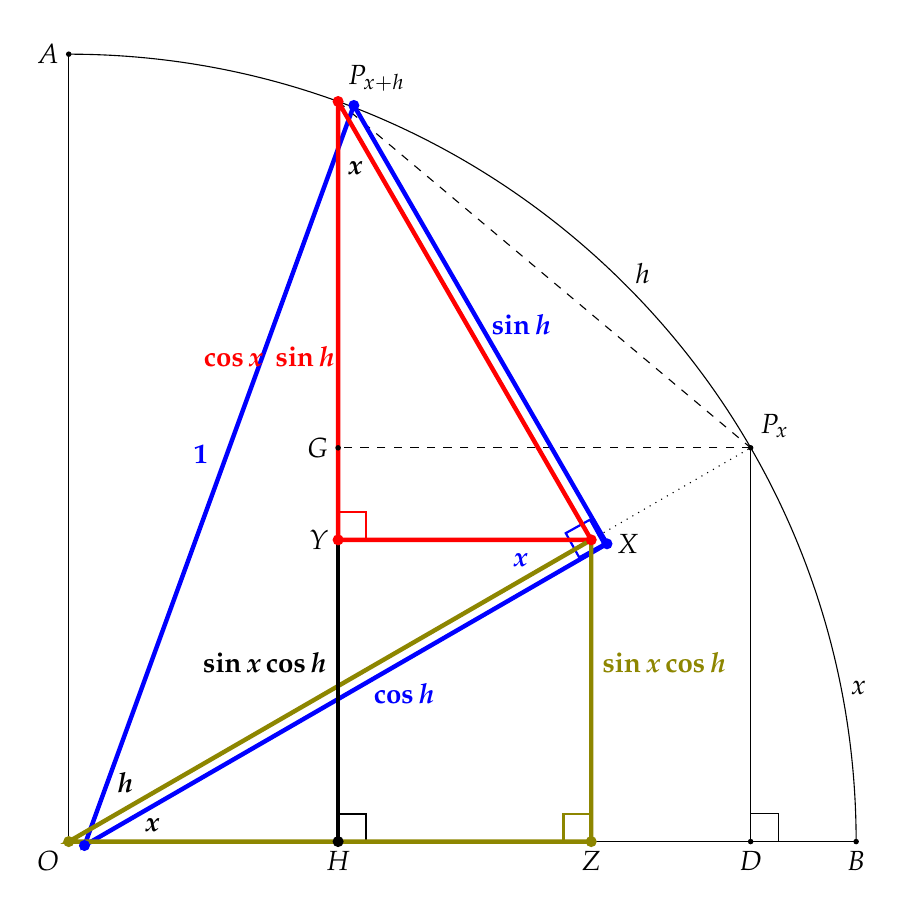
\begin{tikzpicture}[scale=1]
% Coordinate axes, first quadrant
\coordinate (O) at (0,0);
\coordinate (A) at (0,10);
\coordinate (B) at (10,0);
\draw[name path=axes] (B) -- (O) -- (A);

% Arc x+h from 0 to 90
\draw[name path=arc] (10,0)
  arc[start angle=0, end angle=90, radius=10]
  node[very near start,right] {$x$}
  node[midway,right,yshift=4pt] {$h$};

% Ray from origin intersects arc at P_x
\path[name path=px] (O) -- (30:11);
\path [name intersections={of=arc and px,by={Px}}];

% Drop perpendicular from P_x to D
\draw[name path=pxd] (Px) -- (Px |- O);
\path[name intersections={of=pxd and axes,by={D}}];

% Ray from origin intersects arc at P_{x+h}
\path[name path=pxh] (O) -- (70:11);
\path [name intersections={of=arc and pxh,by={Pxh}}];

% Drop perpendicular from P_{x+h} to H
\draw[name path=pxh] (Pxh) -- (Pxh |- O);
\path [name intersections={of=pxh and axes,by={H}}];

% Perpendicular from P_x to P_{x+h}H
\draw[dashed,name path=pxpxh] (Px) -| (Pxh);
\path [name intersections={of=pxh and pxpxh,by={G}}];

% Right angle marks
\draw (D) rectangle +(10pt,10pt);
\draw[thick] (H) rectangle +(10pt,10pt);

% Ray O to P_x, chord P_x to P_{x+h}
\draw[dotted] (O) -- (Px);
\draw[dashed] (Pxh) -- (Px);

% New line segments for proving formula for sin(x+h)

% Drop perpendicular P_{x+h}X  from P_{x+h} to OP_x
%   and draw blue triangle
\coordinate (X) at ($(O)!(Pxh)!(Px)$);
\draw[ultra thick,blue]
  ($(X)+(2mm,-.5mm)$) -- 
    node[below right,xshift=6pt,yshift=8pt] {$\bm{\cos h}$} 
  ($(O)+(2mm,-.5mm)$) --
    node[above left] {$\bm{1}$}
  ($(Pxh)+(2mm,-.5mm)$) --
   node[right] {$\bm{\sin h}$} cycle;
\draw[thick,blue,rotate=119] ($(X)+(-1.2mm,-1.1mm)$) rectangle +(10pt,10pt);

% Drop perpendicular XY from X to P_{x+h}H
%   and draw blue triangle
\draw[ultra thick,red] (Pxh) -- 
   (X) --
      ($(H)!(X)!(Pxh)$) coordinate (Y) 
       -- 
        node[left,red,xshift=3pt,yshift=-13pt]
        {$\bm{\cos x\;\sin h}$} 
      (Pxh);
\draw[thick,red] (Y) rectangle +(10pt,10pt);

% Drop perpendicular from XZ from X to OB 
\draw[ultra thick,olive] (X) -- 
  node[right,yshift=10pt] {$\bm{\sin x \cos h}$} 
    ($(O)!(X)!(B)$) coordinate (Z) --
  (O) -- (X);
\draw[rotate=90,thick,olive] (Z) rectangle +(10pt,10pt);

% Label left side of rectangle
\draw[ultra thick] (H) -- 
  node[left,yshift=10pt] {$\bm{\sin x \cos h}$} (Y);

% Draw intersections of lines
\fill[olive] (O) circle (2pt)
  node[black,below left] {$O$}
  node[black,right,xshift=24pt,yshift=6pt] {$\bm{x}$}
  node[black,above right,xshift=14pt,yshift=14pt] {$\bm{h}$};
\fill (A) circle (1pt) node[left] {$A$};
\fill (B) circle (1pt) node[below] {$B$};
\fill (Px) circle (1pt) node[above right] {$P_x$};
\fill[red] (Pxh) circle (2pt)
  node[black,above right] {$P_{x+h}$}
  node[below right,black,yshift=-18pt] {$\bm{x}$};
\fill (D) circle (1pt) node[below] {$D$};
\fill (H) circle (2pt) node[below] {$H$};
\fill (G) circle (1pt) node[left] {$G$};
\fill[olive] (Z) circle(2pt) node[below,black] {$Z$};
\fill[red] (Y) circle(2pt) node[left,black] {$Y$};
\fill[red] (X) circle(2pt);
\fill[blue] ($(O)+(2mm,-.5mm)$) circle(2pt);
\fill[blue] ($(X)+(2mm,-.5mm)$) circle(2pt)
  node[black,right] {$X$}
  node[below left,xshift=-25pt,yshift=0pt] {$\bm{x}$};
\fill[blue] ($(Pxh)+(2mm,-.5mm)$) circle(2pt);
\end{tikzpicture}
\end{center}
\caption{Proving the formula for $\sin(x+h)$}\label{fig.simple}
\end{figure}



\bibliographystyle{plain}
\bibliography{trigonometric-functions}

\end{document}
